\documentclass[runningheads]{llncs}
\usepackage[T1]{fontenc}

% define lightgray
\usepackage[table]{xcolor}

\usepackage{booktabs}
\usepackage[square,sort,comma,numbers]{natbib}
\usepackage[pdfstartview=XYZ,
bookmarks=true,
colorlinks=true,
linkcolor=blue,
urlcolor=blue,
citecolor=blue,
pdftex,
bookmarks=true,
linktocpage=true, % makes the page number as hyperlink in table of content
hyperindex=true
]{hyperref}

\usepackage{orcidlink} % orcidlink
\usepackage{marvosym} %letter symbol
\usepackage{rotating} % Rotating table
\usepackage{subcaption}
\usepackage{graphicx}
\usepackage{multirow}

\usepackage{amsmath}

\newcommand{\myvec}[1]{\mathbf{#1}}

\newcommand{\jd}[1]{\scriptsize {\bf \color{red}[JD: #1]}\normalsize}

\newcommand{\mn}[1]{\scriptsize {\bf \color{blue}[MN: #1]}\normalsize}


\title{Generating synthetic data is complicated: Know your data and know your generator}
\titlerunning{Generating synthetic data is complicated}

\author{Jonathan Latner\inst{1 (\text{\Letter})\orcidlink{0000-0002-1825-0097}} \and
Marcel Neunhoeffer\inst{1 \orcidlink{0000-0002-9137-5785}}  \and
Jörg Drechsler\inst{1 \orcidlink{0009-0009-5790-3394}}}

\authorrunning{Latner et al., \the\year}

\institute{Institute for Employment Research, Nuremberg, Germany
\email{\{jonathan.latner, marcel.neunhoeffer,joerg.drechsler\}@iab.de}}

\begin{document}

\maketitle              % typeset the header of the contribution

\begin{abstract}
The abstract should briefly summarize the contents of the paper in
150--250 words.

\keywords{First keyword  \and Second keyword \and Another keyword.}
\end{abstract}


\clearpage

% LENGTH OF SUBMISSIONS.

% Using the above format with 11-point font, the paper should be at most 12 pages excluding the bibliography and appendices, and at most 16 pages total. Committee members are not required to read appendices; the paper should be intelligible without them. Submissions not meeting these guidelines risk rejection without consideration of their merits.

\section{Introduction}

\begin{itemize}
    \item \url{Gretel.ai}: The synthetic data platform for developers. Generate artificial datasets with the same characteristics as real data, so you can develop and test AI models without compromising privacy.
    \item \url{Mostly.ai}: Synthetic Data. Better than real. Still struggling with real data? Use existing data for synthetic data generation. Synthetic data is more accessible, more flexible, and simply...smarter.
    \item \url{Statice.ai}: Generating synthetic data comes down to learning the joint probability distribution in an original, real dataset to generate a new dataset with the same distribution.  The more complex the real dataset, the more difficult it is to map dependencies correctly. Deep learning models such as generative adversarial networks (GAN) and variational autoencoders (VAE) are well suited for synthetic data generation.
    \item \url{hazy.com}: Synthetic data does not contain any real data points so can be shared freely. Say goodbye to lengthy governance processes associated with real data.  Specifically, Hazy data is designed to preserve all the patterns, statistical properties and correlations in the source data, so that it can be used as a drop-in replacement for it.
    \item DataSynthesizer: The distinguishing feature of DataSynthesizer is its usability — the data owner does not have to specify any parameters to start generating and sharing data safely and effectively.
\end{itemize}



The idea of releasing synthetic data instead of actual data is often understood to have begun in the early 1990s \cite{rubin1993statistical,little1993statistical}.\footnote{We note that several years before Rubin's seminal paper \cite{rubin1993statistical}, an approach was developed for statistical disclosure protection that we might recognize as synthetic data, but they never called it that way \cite{liew1985data}.}  Here, when we refer to data, we are referring to microdata (i.e. one observation per individual unit) as opposed to tabular data (i.e. summary data).  Releasing synthetic data means fitting a model to the original data and then generating new data based on this model so that the released data do not contain information on a real individual unit (person, firm, etc.) that would reveal information that could be used to identify the unit.  The appeal is that the synthetic data mimic the statistical properties of the original data while maintaining the privacy of individual records.

There is a general perception that making synthetic data are easy.  Our goal is to explain why making synthetic data are complicated.  There are two reasons.  First, one needs to know the data to be synthesized.  Second, one needs to understand the synthetic data generator (SDG).  We illustrate the problems that can result when there is a disconnect between knowledge of the generator and knowledge of the data by using three SDGs and one data set.  In contrast to the simplicity of the original idea, and despite decades of progress, the creation of synthetic data include steps that are neither common knowledge nor described in one place.  Our conclusion: Generating synthetic data is easier than ever. But, to generate good synthetic data, scientists need to have a detailed understanding how and for what purpose the synthetic data are generated.

\section{Study design}\label{sec:study_design}

We compare four measures of utility from three synthetic data generators (SDGs) on one data set.  In section \ref{sec:know_your_data}, we describe the data.  In section \ref{sec:know_your_generator}, we describe the SDGs.  Following Taub et al. \cite{taub2020impact} and Little et al. \cite{little2022comparing}, we assess the utility of the synthetic data using three measures: propensity mean squared error (pMSE), the ratio of estimates (ROE), and confidence interval overlaps (CIO).  These utility measures are implemented in \textsf{R} from the Synthpop package, which we describe later.  We add a fourth measure of utility, the duration in time (in seconds) required to create the synthetic dataset.  Finally, while we do not quantitatively evaluate the privacy of the synthetic data, we qualitatively describe how each SDG approaches privacy in the appropriate subsection.  To obtain consistent results, five fully synthetic datasets were generated using different random seeds for the each original data set.  


{\bf JPL Note: below is direct copy from Little et al., 2022}

According to Little et al. \cite{little2022comparing}, the propensity score, or pMSE, developed in Woo et al. \cite{woo2009global} and Snoke et al. \cite{snoke2018general} is a measure of data utility designed to determine how easy it is to discern between two datasets based upon a classifier. It is calculated by appending the original and synthetic datasets and creating an indicator variable T, where T = 1 for the synthetic dataset and T = 0 for the original dataset. For each record in the combined dataset the probability of being in the synthetic dataset is computed; this is the propensity score. The propensity score can be computed via logistic regression. The distributions of the propensity scores for the original and synthetic data are compared; where these are similar data utility should be high. In summary:

\begin{equation}
pMSE = \frac{1}{N}\sum_{i=1}^{N}[\hat{p}_i - c]^2
\end{equation}

where $N$ is the number of records in the merged dataset, $\hat{p}_i$ is the estimated propensity score for record $i$, and $c$ is the proportion of data in the merged dataset that is synthetic (which is 1/2). A pMSE score close to 0 would indicate high utility (a score of 0 indicates the original and synthetic data are identical).  pMSE can be estimated on the complete data set or subsets of the variables, e.g., all one-way, two-way or three-way combinations.

ROE is calculated by taking the ratio of the synthetic and original data estimates, where the smaller of these two estimates is divided by the larger one. Thus, given two corresponding estimates (e.g. totals, proportions), where $y^1$ is the estimate orig from the original data and $y^1$ is the corresponding estimate from the synthetic synth data, the ROE is calculated as:

\begin{equation}
    ROE = \frac{min(y_{orig}^1,y_{synth}^1)}{max(y_{orig}^1,y_{synth}^1)}
\end{equation}

if $y^1_{orig}=y^1_{synth}$ then the ROE = 1. The ROE will be calculated over univariate data, and takes a value between 0 and 1. For each numerical variable, the ratio of estimates are averaged across binned categories.  For each categorical variable, the ratio of estimates are averaged across categories to give an overall ratio of estimates.

The CIO, proposed by Karr et al. \cite{karr2006framework}, is defined as:

\begin{equation}
    J_k = \frac{1}{2}\left(\frac{U,k-L,k}{U_{orig},k-L_{orig},k} + \frac{U,k-L,k}{U_{syn},k-L_{syn},k}\right)
\end{equation}

where $U,k$ and $L,k$ denote the respective upper and lower bounds of the intersection of the confidence intervals from both the original and synthetic data for estimate $k$, $U_{orig},k$ and $L_{orig},k$ represent the upper and lower bounds of the original data, and $U_{syn},k$ and $L_{syn},k$ of the synthetic data.  Confidence interval overlap from two regression models, one with a dependent variable that is continuous (OLS) and one that is dichotomous (GLM).

Our fourth utility measure is the duration in time (in seconds) required to run one single synthetic dataset, which we refer to as computational efficiency.  

\section{Know your data}\label{sec:know_your_data}

The data we use are called, Social Diagnosis 2011 - Objective and Subjective Quality of Life in Poland (SD2011).  The data are included as part of the Synthpop package.\footnote{We note that the data are publicly available\url{http://www.diagnoza.com/index-en.html}.  However, we are as yet unable to replicate data made available from the Synthpop package from the raw data.}  As shown in table \ref{table:sd2011_data_structure}, there are 35 variables and 5.000 observations.  The data contain 21 variables are categorical (or factor) and 14 variables are numeric.  There are two main reasons why SD2011 data are helpful to illustrate the potential problems that may exist in the disconnect between knowledge of the data and knowledge of the synthetic data generator (SDG).  

One is data dimensionality. Compared to previous evaluations \cite{dankar2021fake,little2022comparing}, SD2011 contain the highest dimensional data set with respect to rows and columns.  While previous research used data with more columns ($> 40$), the data contained far fewer rows ($< 1.000$) or if data contained more rows (32.000), then they contained fewer columns (25).  Further, the data contain a factor variable (\texttt{eduspec}) and a continuous variable (\texttt{wkabdur}) with a large number of unique values.  Data dimensionality affects the duration in time required to generate the synthetic data, which we refer to in this paper as computational efficiency.

The second reason is that SD2011 contain many properties of real data, including missing, `messy' or extreme values, and generated variables.  These properties are both independent and related.  Previous evaluations use clean data from Census or machine learning libraries (Kaggle, UCI, OpenML).  Without denying the value of clean data for evaluation purposes, real data illustrate advantages and disadvantages of SDGs that would otherwise not be understood.

Missing values present several challenges and come in two types: `missing at random' and `informed missings'.  One general problem is that some SDGs cannot be used on data with missing values.  For example, early versions of CTGAN, which we describe later, could not be used on data with missing values.\footnote{\url{https://github.com/sdv-dev/CTGAN/issues/39}}  The ability to synthesize missing values is a stage of development that SDGs must pass through before they can be applied to real data.  

Another general problem is that it is not always clear what values are missing.  For example, factor variables contain missing values and numeric variables contain negative values that we assume are missing.  However, income is a numeric variable that contains both missing and negative values.   

Informed missings present their own challenges.  In its original form \cite{rubin1993statistical}, the idea of creating synthetic data was to treat all data not in a sample as missing data from a population to be filled in using multiple imputation.  The missing data are filled in using models fit with the original data to create synthetic data.  While this approach is not a problem if values are missing at random, it is a problem if missing values are informative.  For example, SD2011 contains a variable for total time spent working abroad (\texttt{wkabdur}) that is missing if an individual did not work abroad (\texttt{wkab} = Y/N).  The correct coding of missing values when creating synthetic data requires knowledge of the data that is not always available and may not be easy to detect or follow simple rules.

Generated variables are variables created from the original values.  In SD2011, there are two generated variables.  The variable \texttt{agegr} is generated from \texttt{age} and the variable \texttt{bmi} is generated from \texttt{height}(cm) and \texttt{weight}(kg).  Given that synthesizing any one variable is a challenge, the challenge increases for each additional variable being synthesized, by definition.  As we will show, the problem is exacerbated when generated variables contain messy or extreme values.  It is not necessary to synthesize generated variables, but generated variables cannot be detected by the SDG and require knowledge of the data that is not always possessed by those with knowledge of the SDG.  

Messy variables also exist.  The variable for \texttt{wkabdur} or `total time spent working abroad' is a numeric variable that Synthpop treats as a factor variable.  Because this variable has a high number of unique values, the treatment of this variable of categorical or continuous affects the duration in time required to synthesize the entire data set.  Another example of messy values are the variables: \texttt{smoke} and \texttt{nociga}.  Two individuals indicate they do not smoke, but also indicate they smoke 20 or 22 cigarettes per day, respectively.  

Finally, while it is easy to label variables as categorical or continuous, some continuous variables can look like categorical variables and visa versa.  For example, the variable for \texttt{nofriend} is a continuous variable for the number of friends a survey respondent has.  As we will show later, values below 10 are normally distributed, but then cluster at 10, 20, and so on.  While it is understood that certain SDGs are more or less appropriate for certain variable types, variation exists within variable types that can also affect utility of a given SDG.  In summary, SD2011 is a useful data set to compare and contrast the advantages and disadvantages of SDGs in a real setting.

We use three versions of the original data to create synthetic data and compare utility.  SD2011(a) is the raw data.  SD2011(b) codes all negative values in numeric variables as missing and all empty values in character variables as missing.  SD2011(c) drops the two generated variables: \texttt{agegr} and \texttt{bmi}.

\section{Know your generator}\label{sec:know_your_generator}

In the beginning, the idea of creating synthetic data was a theoretical process \cite{rubin1993statistical}.  To create synthetic data from actual data, all non-respondents in a survey are treated as missing values to be replaced with `imputed' values.  Given a dataset ($D$) with observations ($n$), there is a two-stage process.  First, a model for predicting a given outcome variable ($y$) given a set of background variables ($x$) is trained on the actual data.  Second, values of the original outcome variable are replaced by random draws from the model of the outcome variable ($y^*$).  This process is then repeated so that all actual values are replaced by imputed values for every variable.  The result is a multiply-imputed synthetic dataset ($D^*$) that contains no values in the actual data, but looks structurally identical to the actual data, not only with respect to mean and variation within a given variable, but also correlations between variables.  

Despite the simplicity, implementing the theoretical process is more complicated than the description might suggest.  One primary question is what method to use.  While the original application may have assumed some sort of parametric estimation using a linear or non-linear model, more recent research borrows from the machine learning literature, including Classification and Regression Trees (CART) \cite{reiter2005using}, Random Forests \cite{caiola2010random}, Support Vector Machines \cite{drechsler2010using}, Bayesian Networks \cite{zhang2017privbayes}, and General Adversarial Networks (GANs) \cite{goodfellow2014generative}, among others.  

A related question is what package to use.  A statistical package that can be loaded into R or Python or another statistical software program that contains a synthetic data generator (SDG) is not the same thing as the method used by the SDG.  For example, the Python package Synthcity \cite{synthcity} contains multiple types of GANs (CTGAN, AdsGan, etc.) and Bayesian (PrivBayes, Bayesian Network) SDGs.  It is important to distinguish the method from the package in order to reduce confusion when evaluating what SDG is right for what type of research question or data.  In this section, we describe tuning the synthetic data generators (SDG).  The focus is on finding optimal utility within a given SDG.  Given the detail, most of the supporting figures are in the respective online appendix.  

\subsection{DataSynthesizer} 

DataSynthesizer (Version 0.1.11) was used \cite{ping2017datasynthesizer}, which implements the PrivBayes algorithm \cite{zhang2017privbayes}.  DataSynthesizer is designed to address the challenges associated with creating synthetic data outputs from high-dimensional real data inputs.  To achieve this goal, the package implements a Bayesian network model, which assumes that all variables are discrete.   When learning a Bayesian network, continuous variables are encoded or discretized and the default value is 20 bins.  Afterward, values are re-encoded within a given bin.  Therefore, the ability to maintain output scalability with dimensionality is partially derived by sacrificing some amount of utility in continuous variables.   

There are a number of hyperparameters that might be tuned for DataSynthesizer, but we focus on two, with all other values set to default.  One hyperparemeter is differential privacy ($\epsilon$-DP). This is a number that quantifies the amount of noise that is introduced into the original data to create synthetic data.  In Datasynthesizer, the default is 0.1 and 0 turns off DP.  We turn off DP in order to compare to the other synthesizers that do not have a similar hyperparameter.  

A second hyperparameter are the number of attributes any one variable can have, i.e. parents ($k$).  In a Bayesian Network, there are three possible relationships between X and Y.  Direct dependence where each variable can only have direct attributes (1 parent), weak conditional independence where each variable can have both direct and indirect attributes (2+ parents), and strong conditional independence where all variables are independent (0 parents).  

As a first step, we tune DataSynthesizer based on the number of parents in the Bayesian network using pMSE as a utility measure using SD2011(a), as shown in figure \ref{fig:tuning_ds_dataset} in the online appendix \ref{appendix:datasynethsizer}.  The utility measure is the pMSE and pMSE = 0.25 for 0 and 1 parents; pMSE = 0.2 with 2 parents; and pMSE = 0.21 for 3 parents.  Therefore, 2 parents represents the optimal level of utility.

Next, we estimate pMSE for all two-way combinations of variables in SD2011(a), as shown in figure \ref{subfig:ds_fidelity_two_way_subfig-a}.  While most values are close to 0, it is clear that synthetic values do not match well with original values for the variable, \texttt{wkabdur} (work abroad duration).  In the original data, 0.975\% of all values are -8, as shown in figure \ref{subfig:ds_variable_wkabdur}.  The problem is that DataSynthesizer not only creates synthetic values of -8, but also values between -8 and 0 that do not exist in the original data.  Therefore, we code all negative values in numeric variables as missing and all empty values in character variables as missing, this is SD2011(b).

Next, we re-estimate pMSE for all two-way combinations of variables in SD2011(b), as shown in figure \ref{subfig:ds_fidelity_two_way_subfig-b}.  While most values are close to 0, it is clear that synthetic values do not match well with original values for the variable, \texttt{bmi} (body mass index).  In the original data, the variable \texttt{bmi} contains a single value of 450, as shown in figure \ref{subfig:ds_variable_bmi}.  This is an extreme value that is nearly 6 times larger than the next closest value of 76.  Similar to the variable, \texttt{wkabdur}, the problem is that DataSynthesizer not only creates synthetic values of 450, but also values between 76 and 450 that do not exist in the original data.  Therefore, we drop both generated variables (\texttt{bmi} and \texttt{agegr}) to create SD2011(c).

In summary, this exercise illustrates two key points.  First, one must know the generator.  The Bayesian network implemented by DataSynthesizer discretizes continuous variables into bins and then re-encodes values within a given bin.  Second, one must know the data.  Missing/negative or extreme values as well as the presence of generated variables affect the similarity or difference between the synthetic and original data.  If we compare pMSE across the three versions of SD2011, then  pMSE = 0.21 for SD2011(a), pMSE = 0.13 for SD2011(b), and pMSE = 0.07 for SD2011(c), as shown in figure \ref{fig:tuning_ds_optimize_dataset_compare}.  Therefore, preprocessing the data is at least as important, if not more than tuning the synthesizer.

\subsection{CTGAN} 

CTGAN (Version 1.9.0) was used \cite{ctgan}.  CTGAN is part of the Synthetic Data Vault package \cite{patki2016synthetic}.  GANs \cite{goodfellow2014generative} simultaneously train two neural networks: a generator and a discriminator. The generator aims to create synthetic data that becomes increasingly indistinguishable from original data.  The discriminator tries to get better at distinguishing between original and synthetic data.  This adversarial process goes back and forth until the discriminator cannot distinguish between the original data and the generated data.  

In their original application, GANs were designed to create synthetic images, but the approach was adapted to create synthetic microdata.  One advantage is that GANs were created to deal with continuous variables (unlike DataSynthesizer).  The disadvantage is that cells in micro data are not informative of neighbors in the same way that pixel cells in a photograph. As a result, GANs can struggle modeling relationships between cells and columns \cite{drechsler202330}.

CTGAN contains a number of hyperparameters that one can use to tune the model. Following the package authors, we refer to these as `primary' and `advanced'.  The primary one is the number of steps contained in the model, which is a function of the number of observations in the original data and two hyperparameters: Epochs and Batch size.  In the default, batch size is 500 and epochs is 300.  With 5.000 observations in the original data, this means that it takes 10 steps within each Epoch to examine the entire data frame (5000/500=10) and the total number of steps is 3.000 (10*300).  Too few epochs may result in underfitting and too many epochs may result in overfitting.

Advanced hyperparameters include dimensionality and embedding dimension, but others exist (i.e learning rate, and weight decay, etc.).  The dimensionality is the number of layers in the generator/discriminator networks.  A fully connected layer will be created for each one of the values provided (default is [256,256]).  Technically, one can vary the values for both the dimensionality of the discriminator and generator, but we set the same value for both.  The embedding dimension influences how much the information in the original data set is compressed.  For example, an embedding dimension of 1 is equivalent to storing 34 columns of data in SD2011(c) in a single number (default is 128).

As shown in figure \ref{fig:ctgan_fidelity_optimize} in online Appendix \ref{appendix:CTGAN}, we tune the hyperparameters in three main ways.  First, we maintain a constant number of steps (3.000), but allow the batch size to vary (figure \ref{subfig:ctgan_fidelity_optimize_batch_size}).  Second, we maintain a constant batch size (500), but allow the steps to vary (figure \ref{subfig:ctgan_fidelity_optimize_epochs}).  Third and finally, we vary the dimensionality of the generator/discriminator networks and the embedding dimension (figure \ref{subfig:ctgan_fidelity_optimize_dimensions}).  Surprisingly, tuning these hyperparameters makes little difference with pMSE around 0.16.  Given that, we maintain default values for all hyperparameters with the exception of epochs, which we increase to 600.

In summary, this exercise illustrates two key points.  First, tuning CTGAN made little difference in the utility of the synthetic data.  We are aware of other, similar research (as yet unpublished) where tuning CTGAN did make a difference.  One possible explanation is that our data contain a relatively small number of observations (5.000).  Second, we note that pMSE is about twice as high as our optimized SDG using DataSynthesizer.  The interpretation is that CTGAN is not a very good synthesizer.  However, as described earlier, CTGAN is not the only GAN one can use to create synthetic microdata.  Evidence (unpublished) suggests it is possible to create a better GAN.

\subsection{Synthpop} 

Synthpop (Version 1.8.0) \cite{nowok2016synthpop} was used. Synthpop is an R package that implements parametric and CART models (classification and regression trees) to generate synthetic data.  CART models are the default.  According to the online description,\footnote{\url{https://www.synthpop.org.uk/about-synthpop.html\#methodology}} Synthpop follows the two-stage process described by Rubin \citep{rubin1993statistical}, where the data are synthesized one at a time using sequential regression modelling.  

Evaluations often find that Synthpop/CART models appear to create synthetic data that are statistically more similar to original data  \cite{little2022comparing,dankar2021fake,drechsler2011empirical}.  However, Synthpop, like all SDGs contains advantages and disadvantages \cite{little2022comparing}.  The advantage is one can easily create synthetic data with high levels of utility and little tuning, but the disadvantage is that CART and tree-based models in general struggle computationally with variables that contain many categories.  For this reason, we use default values of Synthpop.


\section{Comparing SDGs}\label{sec:results}

In this section, we compare our three synthetic data generators (SDGs) on our four measures of utility.  We begin by comparing pMSE across our optimized SDGs, as shown in figure \ref{subfig:graph_fidelity_compare_dataset}.  pMSE = 0.15 for CTGAN, 0.07 for DataSynthesizer, and 0.02 for Synthpop.  More detail is visible in figure  \ref{subfig:graph_fidelity_compare_twoway} that compares two-way pMSE for all variables in the data.  In Synthpop, values are close to zero for most variables.  In CTGAN, values are close to 0.075 for most variables.  In DataSynthesizer, values are close to zero for most variables except the variable, \texttt{nofriend} (number of friends).  The overall interpretation is that synthetic data from Synthpop is much closer to the original data (SD2011c) than synthetic data from CTGAN or DataSynthesizer.

Next, we examine one-way frequency statistics and the ratio of estimates (ROE) for select variables to better understand how different SDGs estimate synthetic values, as shown in figure \ref{fig:graph_frequency_compare}.  We begin with  the variable, \texttt{nofriend} (number of friends), as shown in \ref{subfig:graph_frequency_compare_nofriend}.  In the original data, the variable \texttt{nofriend} is a continuous variables that are normally distributed below 10, but then clusters at values of 10, 15, 20 and groups of 10 up to the maximum 99.  In values below 30, Synthpop and CTGAN perform similarly well, but DataSynthesizer does not capture clustering or discontinuity in the variable.  Instead, DataSynthesizer replaces real values with values that are normally distributed.  In values above 30, CTGAN and DataSynthesizer are similarly bad.  If we examine ROE values for the variable  \texttt{nofriend} from figure \ref{subfig:graph_compare_roe}, then ROE = 0.4 for Synthpop, ROE = 0.28 for CTGAN, and 0.17 for DataSynthesizer (higher values are better).  In both values above and below 30, Synthpop is the only SDG to capture the discontinuity in the continuous variable.  

We get a different picture of SDG quality when we look at the variable, \texttt{bmi} (Body mass index), as shown in figure \ref{subfig:graph_frequency_compare_bmi}.  BMI is normally distributed and ROE = 0.21 for both CTGAN and DataSynthesizer, and ROE = 0.24 for Synthpop.  Therefore, even if Synthpop is slightly better, all three SDGs similarly capture the normally distributed variable of BMI.  

The last variable we examine is \texttt{wkabdur} (Work abroad duration).  Values refer to the number of weeks a survey respondent worked abroad between 2007 and 2011, as shown in figure \ref{subfig:graph_frequency_compare_wkabdur}.  Nearly 98\% of all values are missing, indicating that a respondent did not work abroad.  Interestingly, both Synthpop and CTGAN overestimate the median as 14, but in the original data the mean is 14 and the median is 10.  However, Synthpop is still better at capturing the distribution of the small number of nonmissing values than DataSynthesizer.

Figure \ref{fig:utility_compare_cio} displays parameter estimates and confidence interval overlap (CIO) for two regression models, an OLS model where the dependent variable is \texttt{LN(Income)} and a GLM model where the dependent variable is \texttt{smoke}.  In both models, the independent variables are \texttt{gender}, \texttt{age}, \texttt{education}, and \texttt{bmi}.  In both models, Synthpop has the highest percent of CIO with CTGAN and DataSynthesizer perform similarly badly.  However, when we examine the parameter estimates from the GLM model, Synthpop, like CTGAN and DataSynthesizer, over estimates the effect of education level on smoking for two values: less than secondary and secondary.  Therefore, while synthetic data from Synthpop better capture parametric relationships in the original data, they are not a substitute for real data.

Finally, we compare the duration in time required to create synthetic data from the SDGs, i.e. computational efficiency, as shown in table \ref{table:table_sd2011_duration}.  The first row displays results from the raw data.  CTGAN requires 331 seconds (5 minutes and 30 seconds) and DataSynthesizer requires 245 seconds (4 minutes).  By contrast, duration times from Synthpop are much longer.  If we load SD2011 into R as a .csv file as we do with DataSynthesizer and CTGAN, then Synthpop requires 2.132 seconds (35 minutes and 30 seconds), but we if load SD2011 into R from the Synthpop package, then Synthpop requires 5.474 seconds (91 minutes).

The difference in duration within Synthpop and between Synthpop and the other SDGs is explained by two variables: \texttt{eduspec} and \texttt{wkabdur}.  Both variables are variables with a large number of unique values (28 and 33, respectively).  For some reason when SD2011 is loaded into R from the Synthpop package, then \texttt{wkabdur} is treated as a character variable, not a numeric variable, as it actually is.  However, if SD2011 is loaded into R from a .csv file, then \texttt{wkabdur} is correctly treated as a numeric variable.  The second problem is that Synthpop struggles computationally with variables that contain many categories.  A suggestion is to place this variables at the end prior to synthesizing the data \cite{raab2017guidelines}.  When we treat \texttt{wkabdur} as a numeric variable and place \texttt{eduspec} at the end, then Synthpop requires less than 15 seconds, regardless of how SD2011 is loaded.  Therefore, Synthpop is more computationally efficient with SD2011 than either CTGAN or DataSynthesizer with proper preprocessing.

However, the issue reveals a more general problem: unlike CTGAN and DataSynthesizer, Synthpop is sensitive to the number (and order) of categorical variables with large values.  To illustrate this, we added one, two, or three categorical variables with 20, 25, or 30 unique random values to SD2011.  While duration times for CTGAN and DataSynthesizer are almost insensitive to the number of categorical variables or unique values, duration times for Synthpop increase with additional variable and number of unique values.  Therefore, Synthpop is less computationally efficient as the data dimensions increase.


\section{Conclusion}\label{sec:conclusion}

The key conclusion is that making synthetic data is complicated because it requires knowledge that may not always exist in one place.  

know your data

utility vs. computational efficiency

CTGAN is not good, but other GANs may be better



There is no one size fits all solution and choosing the right synthetic data generator (SDG) is the result of different trade-offs



\subsubsection*{Acknowledgments}
Use unnumbered third level headings for the acknowledgments. All acknowledgments, including those to funding agencies, go at the end of the paper. Only add this information once your submission is accepted and deanonymized. 

%%%%%%%%%%%%%%%%%%%%%%%%%%%%%%%%
% Tables
%%%%%%%%%%%%%%%%%%%%%%%%%%%%%%%%
\clearpage
\section{Tables}

\vskip -5mm
\begin{table}[!htb]
\minipage{\textwidth}
% \begin{table}
    \caption{Social Diagnosis 2011 (SD2011)}
    \centering
    \rowcolors{1}{white}{lightgray}
    \resizebox{\textwidth}{!}{% latex table generated in R 4.4.0 by xtable 1.8-4 package
% Thu Sep 26 09:11:53 2024
\begin{tabular}{rlllllllll}
  \toprule
Number & Variable & Description & Type & Observations & Unique.Values & Missings & Negative.values & Generated & Messy \\ 
  \midrule
  1 & sex & Sex & factor & 5000 & 2 & 0 & 0 &  &  \\ 
    2 & age & Age of person, 2011 & numeric & 5000 & 79 & 0 & 0 &  &  \\ 
    3 & agegr & Age group, 2011 & factor & 5000 & 7 & 4 & 0 & Yes & Yes \\ 
    4 & placesize & Category of the place of residence & factor & 5000 & 6 & 0 & 0 &  &  \\ 
    5 & region & Region (voivodeship) & factor & 5000 & 16 & 0 & 0 &  &  \\ 
    6 & edu & Highest educational qualification, 2011 & factor & 5000 & 5 & 7 & 0 &  &  \\ 
    7 & eduspec & Discipline of completed qualification & factor & 5000 & 28 & 20 & 0 &  &  \\ 
    8 & socprof & Socio-economic status, 2011 & factor & 5000 & 10 & 33 & 0 &  &  \\ 
    9 & unempdur & Total duration of unemployment in the last 2 years (in months) & numeric & 5000 & 30 & 0 & 1556 &  &  \\ 
   10 & income & Personal monthly net income & numeric & 5000 & 407 & 683 & 603 &  & Yes \\ 
   11 & marital & Marital status & factor & 5000 & 7 & 9 & 0 &  &  \\ 
   12 & mmarr & Month of marriage & numeric & 5000 & 13 & 1350 & 0 &  &  \\ 
   13 & ymarr & Year of marriage & numeric & 5000 & 75 & 1320 & 0 &  &  \\ 
   14 & msepdiv & Month of separation/divorce & numeric & 5000 & 13 & 4300 & 0 &  &  \\ 
   15 & ysepdiv & Year of separation/divorce & numeric & 5000 & 51 & 4275 & 0 &  &  \\ 
   16 & ls & Perception of life as a whole & factor & 5000 & 8 & 8 & 0 &  &  \\ 
   17 & depress & Depression symptoms indicator & numeric & 5000 & 23 & 89 & 0 &  &  \\ 
   18 & trust & View on interpersonal trust & factor & 5000 & 4 & 37 & 0 &  &  \\ 
   19 & trustfam & Trust in own family members & factor & 5000 & 4 & 11 & 0 &  &  \\ 
   20 & trustneigh & Trust in neighbours & factor & 5000 & 4 & 11 & 0 &  &  \\ 
   21 & sport & Active engagement in some form of sport or exercise & factor & 5000 & 3 & 41 & 0 &  &  \\ 
   22 & nofriend & Number of friends & numeric & 5000 & 44 & 0 & 41 &  & Yes \\ 
   23 & smoke & Smoking cigarettes & factor & 5000 & 3 & 10 & 0 &  &  \\ 
   24 & nociga & Number of cigarettes smoked per day & numeric & 5000 & 30 & 0 & 3737 &  & Yes \\ 
   25 & alcabuse & Drinking too much alcohol & factor & 5000 & 3 & 7 & 0 &  &  \\ 
   26 & alcsol & Starting to use alcohol to cope with troubles & factor & 5000 & 3 & 82 & 0 &  &  \\ 
   27 & workab & Working abroad in 2007-2011 (in months) & factor & 5000 & 3 & 438 & 0 &  &  \\ 
   28 & wkabdur & Total time spent on working abroad & numeric & 5000 & 33 & 0 & 4875 &  & Yes \\ 
   29 & wkabint & Plans to go abroad to work in the next two years & factor & 5000 & 4 & 36 & 0 &  &  \\ 
   30 & wkabintdur & Intended duration of working abroad & factor & 5000 & 6 & 4697 & 0 &  &  \\ 
   31 & emcc & Intended destination country & factor & 5000 & 18 & 4714 & 0 &  &  \\ 
   32 & englang & Knowledge of English language & factor & 5000 & 4 & 15 & 0 &  &  \\ 
   33 & height & Height of person & numeric & 5000 & 65 & 35 & 0 &  &  \\ 
   34 & weight & Weight of person & numeric & 5000 & 91 & 53 & 0 &  &  \\ 
   35 & bmi & Body mass index (weight - kg/(height - cm$^2$)*10000) & numeric & 5000 & 1396 & 59 & 0 & Yes & Yes \\ 
   \bottomrule
\end{tabular}
}
    % % latex table generated in R 4.4.0 by xtable 1.8-4 package
% Thu Sep 26 09:11:53 2024
\begin{tabular}{rlllllllll}
  \toprule
Number & Variable & Description & Type & Observations & Unique.Values & Missings & Negative.values & Generated & Messy \\ 
  \midrule
  1 & sex & Sex & factor & 5000 & 2 & 0 & 0 &  &  \\ 
    2 & age & Age of person, 2011 & numeric & 5000 & 79 & 0 & 0 &  &  \\ 
    3 & agegr & Age group, 2011 & factor & 5000 & 7 & 4 & 0 & Yes & Yes \\ 
    4 & placesize & Category of the place of residence & factor & 5000 & 6 & 0 & 0 &  &  \\ 
    5 & region & Region (voivodeship) & factor & 5000 & 16 & 0 & 0 &  &  \\ 
    6 & edu & Highest educational qualification, 2011 & factor & 5000 & 5 & 7 & 0 &  &  \\ 
    7 & eduspec & Discipline of completed qualification & factor & 5000 & 28 & 20 & 0 &  &  \\ 
    8 & socprof & Socio-economic status, 2011 & factor & 5000 & 10 & 33 & 0 &  &  \\ 
    9 & unempdur & Total duration of unemployment in the last 2 years (in months) & numeric & 5000 & 30 & 0 & 1556 &  &  \\ 
   10 & income & Personal monthly net income & numeric & 5000 & 407 & 683 & 603 &  & Yes \\ 
   11 & marital & Marital status & factor & 5000 & 7 & 9 & 0 &  &  \\ 
   12 & mmarr & Month of marriage & numeric & 5000 & 13 & 1350 & 0 &  &  \\ 
   13 & ymarr & Year of marriage & numeric & 5000 & 75 & 1320 & 0 &  &  \\ 
   14 & msepdiv & Month of separation/divorce & numeric & 5000 & 13 & 4300 & 0 &  &  \\ 
   15 & ysepdiv & Year of separation/divorce & numeric & 5000 & 51 & 4275 & 0 &  &  \\ 
   16 & ls & Perception of life as a whole & factor & 5000 & 8 & 8 & 0 &  &  \\ 
   17 & depress & Depression symptoms indicator & numeric & 5000 & 23 & 89 & 0 &  &  \\ 
   18 & trust & View on interpersonal trust & factor & 5000 & 4 & 37 & 0 &  &  \\ 
   19 & trustfam & Trust in own family members & factor & 5000 & 4 & 11 & 0 &  &  \\ 
   20 & trustneigh & Trust in neighbours & factor & 5000 & 4 & 11 & 0 &  &  \\ 
   21 & sport & Active engagement in some form of sport or exercise & factor & 5000 & 3 & 41 & 0 &  &  \\ 
   22 & nofriend & Number of friends & numeric & 5000 & 44 & 0 & 41 &  & Yes \\ 
   23 & smoke & Smoking cigarettes & factor & 5000 & 3 & 10 & 0 &  &  \\ 
   24 & nociga & Number of cigarettes smoked per day & numeric & 5000 & 30 & 0 & 3737 &  & Yes \\ 
   25 & alcabuse & Drinking too much alcohol & factor & 5000 & 3 & 7 & 0 &  &  \\ 
   26 & alcsol & Starting to use alcohol to cope with troubles & factor & 5000 & 3 & 82 & 0 &  &  \\ 
   27 & workab & Working abroad in 2007-2011 (in months) & factor & 5000 & 3 & 438 & 0 &  &  \\ 
   28 & wkabdur & Total time spent on working abroad & numeric & 5000 & 33 & 0 & 4875 &  & Yes \\ 
   29 & wkabint & Plans to go abroad to work in the next two years & factor & 5000 & 4 & 36 & 0 &  &  \\ 
   30 & wkabintdur & Intended duration of working abroad & factor & 5000 & 6 & 4697 & 0 &  &  \\ 
   31 & emcc & Intended destination country & factor & 5000 & 18 & 4714 & 0 &  &  \\ 
   32 & englang & Knowledge of English language & factor & 5000 & 4 & 15 & 0 &  &  \\ 
   33 & height & Height of person & numeric & 5000 & 65 & 35 & 0 &  &  \\ 
   34 & weight & Weight of person & numeric & 5000 & 91 & 53 & 0 &  &  \\ 
   35 & bmi & Body mass index (weight - kg/(height - cm$^2$)*10000) & numeric & 5000 & 1396 & 59 & 0 & Yes & Yes \\ 
   \bottomrule
\end{tabular}

    \label{table:sd2011_data_structure}
% \end{table}
\endminipage

\vskip 5mm
\minipage{\textwidth}
% \begin{table}
    \caption{Ratio of estimates (ROE)}
    \centering
    \rowcolors{1}{white}{lightgray}
    \resizebox{.5\textwidth}{!}{% latex table generated in R 4.3.2 by xtable 1.8-4 package
% Wed May  1 12:47:00 2024
\begin{tabular}{lrrr}
  \toprule
variable & ctgan & datasynthesizer & synthpop \\ 
  \midrule
BMI & 0.21 & 0.21 & 0.24 \\ 
  Education & 0.88 & 0.99 & 0.94 \\ 
  Number of friends & 0.28 & 0.17 & 0.40 \\ 
  Work abroad duration & 0.06 & 0.29 & 0.38 \\ 
   \bottomrule
\end{tabular}
}
    \label{table:table_compare_roe}
% \end{table}
\endminipage

\vskip 5mm
\minipage{\textwidth}
% \begin{table}
    \centering
    \caption{Duration (in seconds)}
    \rowcolors{1}{white}{lightgray}
    \resizebox{\textwidth}{!}{% latex table generated in R 4.4.0 by xtable 1.8-4 package
% Fri Jul 19 16:14:31 2024
\begin{tabular}{llrrrr}
  \toprule
version & description & ctgan & datasynthesizer & synthpop (csv) & synthpop (package) \\ 
  \midrule
v00 & Raw (SD2011) & 331.01 & 245.37 & 2132.12 & 5474.39 \\ 
  v01 & Without eduspec or wkabdur & 290.30 & 264.43 & 10.99 & 8.45 \\ 
  v02 & Without wkabdur & 337.07 & 351.76 & 13.96 & 11.02 \\ 
  v03 & Without eduspec & 306.46 & 351.24 & 11.39 & 8.92 \\ 
  v04 & Last variables: eduspec-wkabdur & 374.57 & 344.02 & 14.23 & 287.85 \\ 
  v05 & Last variables: wkabdur-eduspec & 419.60 & 339.92 & 14.60 & 3657.55 \\ 
  v06 & as.numeric(wkabdur) and last variable: eduspec & 356.02 & 347.36 & 14.12 & 11.05 \\ 
  v07\_1\_20 & + 1 factor variable (20 values) & 339.05 & 264.96 & 42.23 &  \\ 
  v07\_1\_25 & + 1 factor variable (25 values) & 400.28 & 326.84 & 137.47 &  \\ 
  v07\_1\_30 & + 1 factor variable (30 values) & 339.73 & 269.72 & 363.18 &  \\ 
  v07\_2\_20 & + 2 factor variable (20 values) & 369.74 & 339.45 & 74.96 &  \\ 
  v07\_2\_25 & + 2 factor variable (25 values) & 364.56 & 361.81 & 631.43 &  \\ 
  v07\_2\_30 & + 2 factor variable (30 values) & 373.25 & 346.15 & 1222.54 &  \\ 
  v07\_3\_20 & + 3 factor variable (20 values) & 393.99 & 369.58 & 122.77 &  \\ 
  v07\_3\_25 & + 3 factor variable (25 values) & 401.03 & 383.40 & 881.53 &  \\ 
  v07\_3\_30 & + 3 factor variable (30 values) & 394.44 & 424.64 & 3654.59 &  \\ 
   \bottomrule
\end{tabular}
}
    \label{table:table_sd2011_duration}
    \\
    \raggedright
    \tiny{Notes: Synthpop (csv) indicates that SD2011 was loaded into R from a csv file.  Synthpop (package) indicates that SD2011 was loaded into R from the Synthpop package.}
% \end{table}
\endminipage
\end{table}

%%%%%%%%%%%%%%%%%%%%%%%%%%%%%%%%
% Graphs
%%%%%%%%%%%%%%%%%%%%%%%%%%%%%%%%
\clearpage
%%%%%%%%%%%%%%%%%%%%%%%%%%%%%%%%%%%%%%
% Graphs
%%%%%%%%%%%%%%%%%%%%%%%%%%%%%%%%%%%%%%
\clearpage
\section{Graphs}

\begin{figure}[ht]
    \caption{Comparing Synthetic Data Generators (pMSE)}
    \label{fig:graph_fidelity_compare}
    \centering

    \begin{subfigure}{\textwidth}
        \caption{pMSE}
        \resizebox{\textwidth}{!}{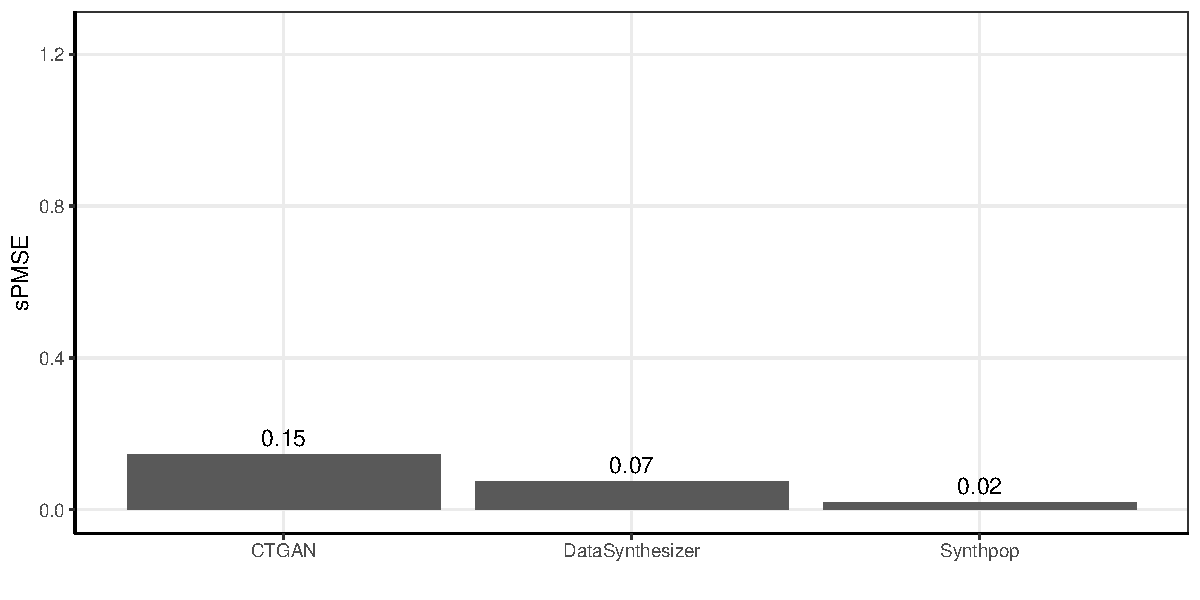
\includegraphics{../graphs/graph_fidelity_compare_dataset.pdf}}
        \label{subfig:graph_fidelity_compare_dataset}
    \end{subfigure}

    \begin{subfigure}{\textwidth}
        \caption{Two-way pMSE}
        \resizebox{\textwidth}{!}{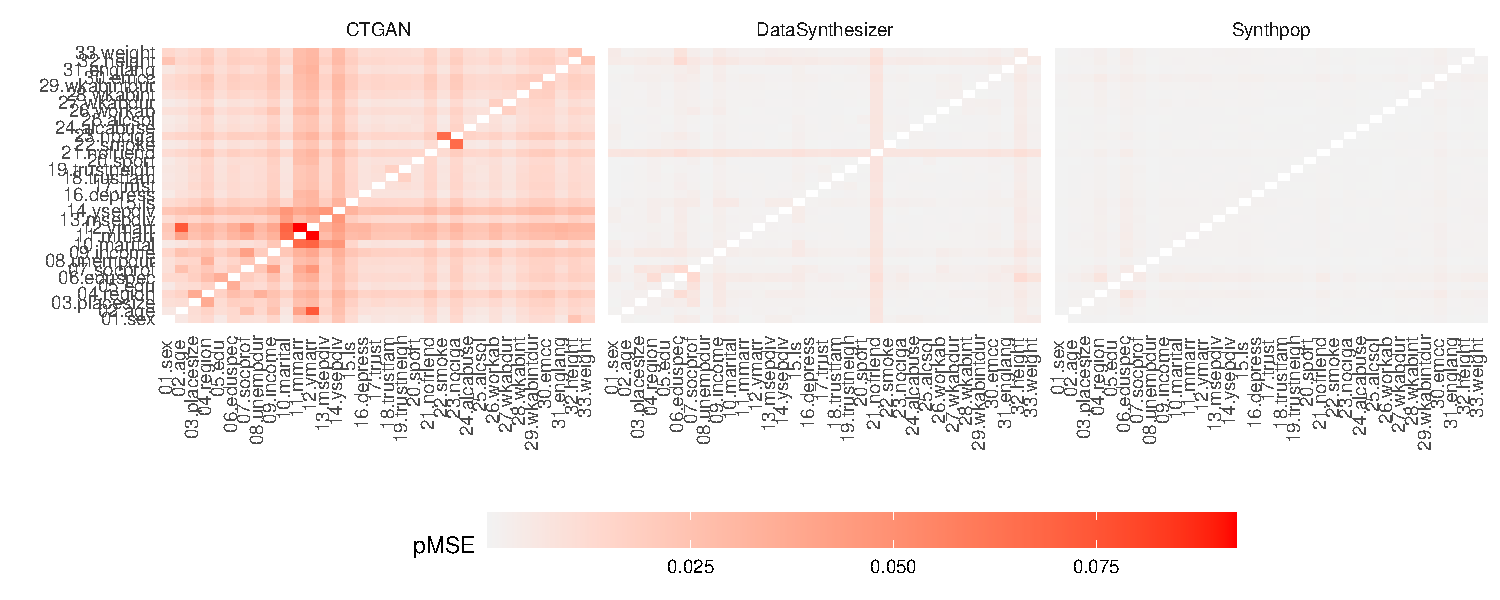
\includegraphics{../graphs/graph_fidelity_twoway_compare.pdf}}
        \label{subfig:graph_fidelity_compare_twoway}
    \end{subfigure}
\end{figure}


\begin{figure}[ht]
    \caption{Comparing one-way frequency of select variables and ROE}
    \label{fig:graph_frequency_compare}
    \centering

    \begin{subfigure}{\textwidth}
        \centering        
        \caption{Number of friends}
        \resizebox{.9\textwidth}{!}{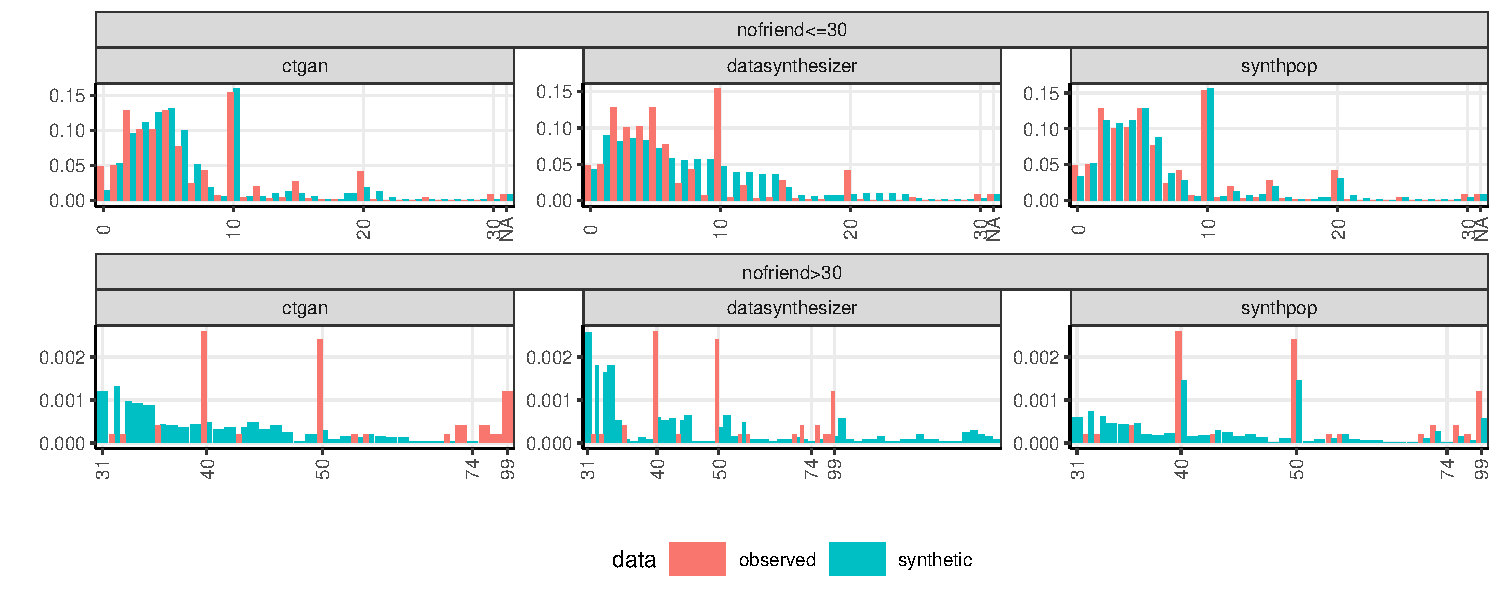
\includegraphics{../graphs/compare_nofriend_1.pdf}}
        \label{subfig:graph_frequency_compare_nofriend}
    \end{subfigure}

    \begin{subfigure}{\textwidth}
        \centering        
        \caption{BMI}
        \resizebox{.9\textwidth}{!}{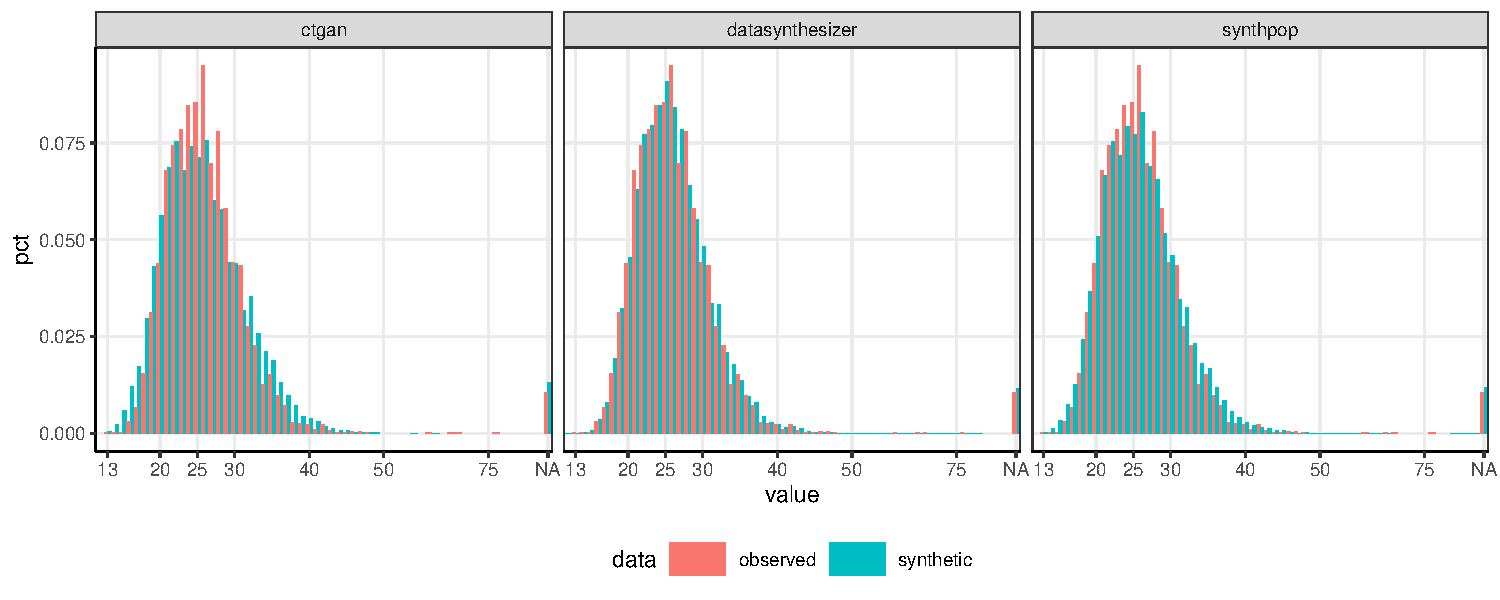
\includegraphics{../graphs/compare_bmi_1.pdf}}
        \label{subfig:graph_frequency_compare_bmi}
    \end{subfigure}

    \begin{subfigure}{\textwidth}
        \centering        
        \caption{Work abroad duration}
        \resizebox{.9\textwidth}{!}{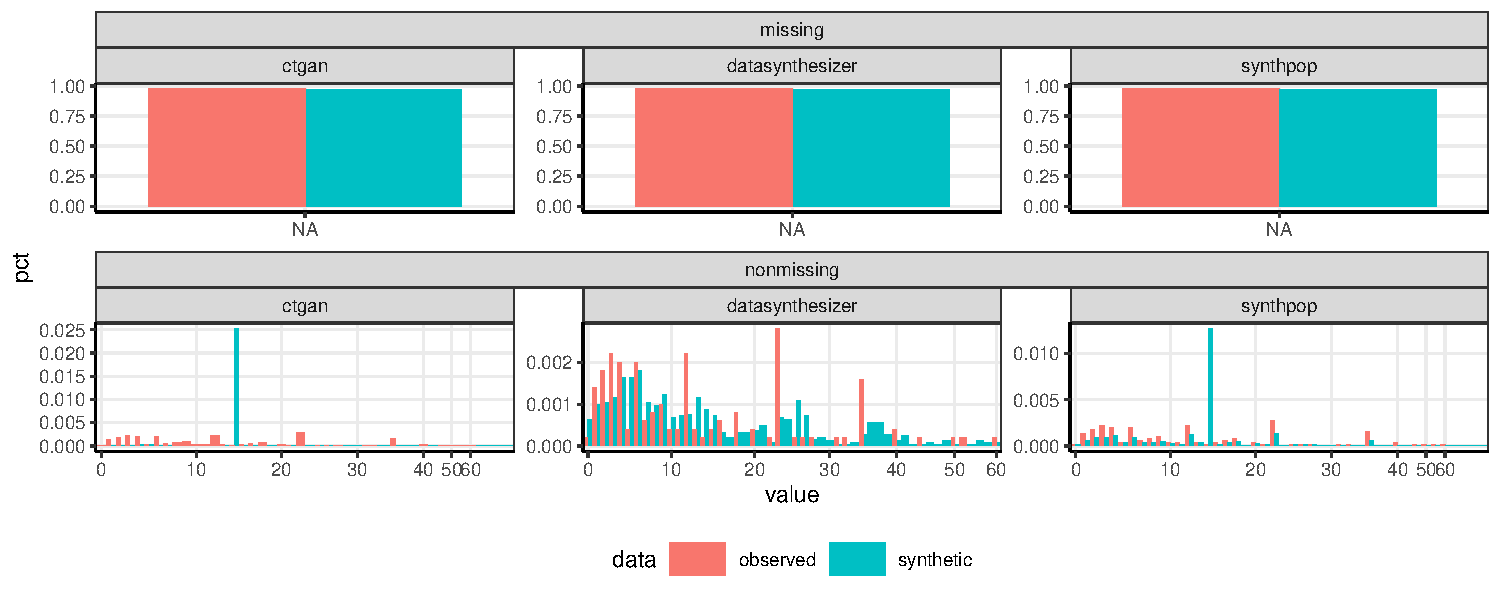
\includegraphics{../graphs/compare_wkabdur_1.pdf}}
        \label{subfig:graph_frequency_compare_wkabdur}
    \end{subfigure}

    \begin{subfigure}{\textwidth}
        \centering        
        \caption{Ratio of estimates (ROE)}
        \resizebox{.9\textwidth}{!}{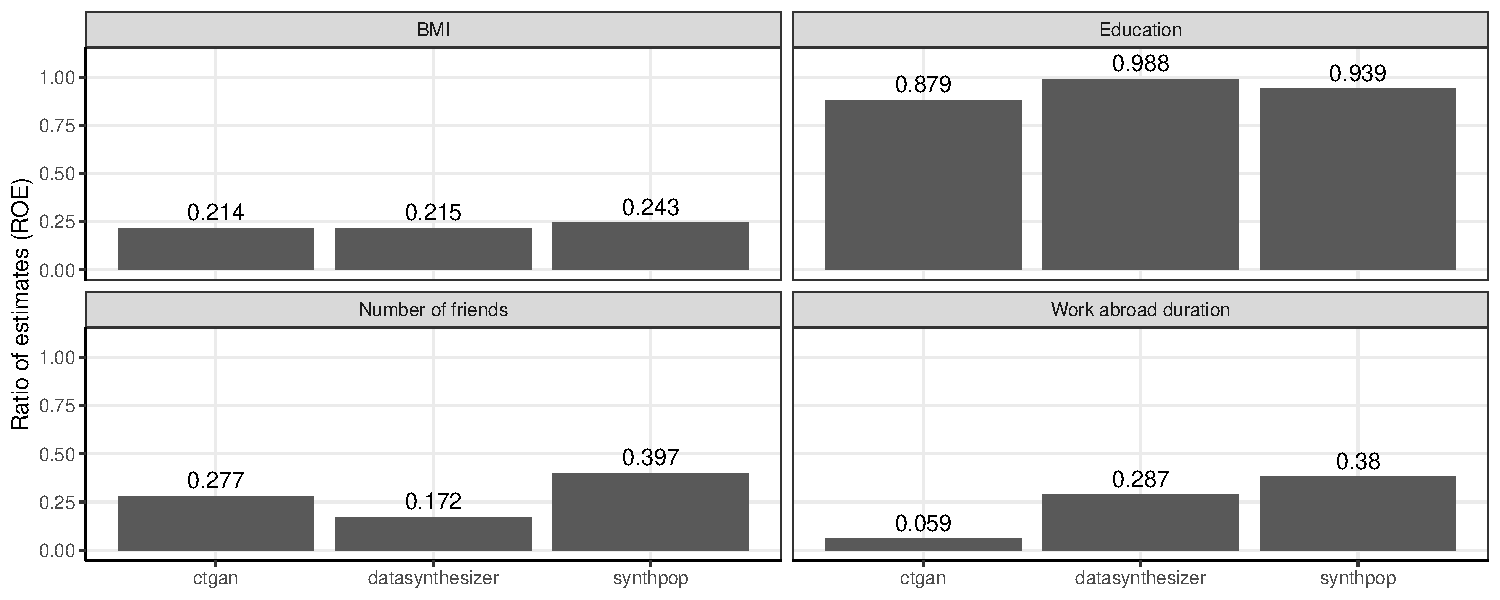
\includegraphics{../graphs/graph_compare_roe.pdf}}
        \label{subfig:graph_compare_roe}
    \end{subfigure}
\end{figure}

\begin{figure}
    \caption{Confidence interval overlap}
    \resizebox{\textwidth}{!}{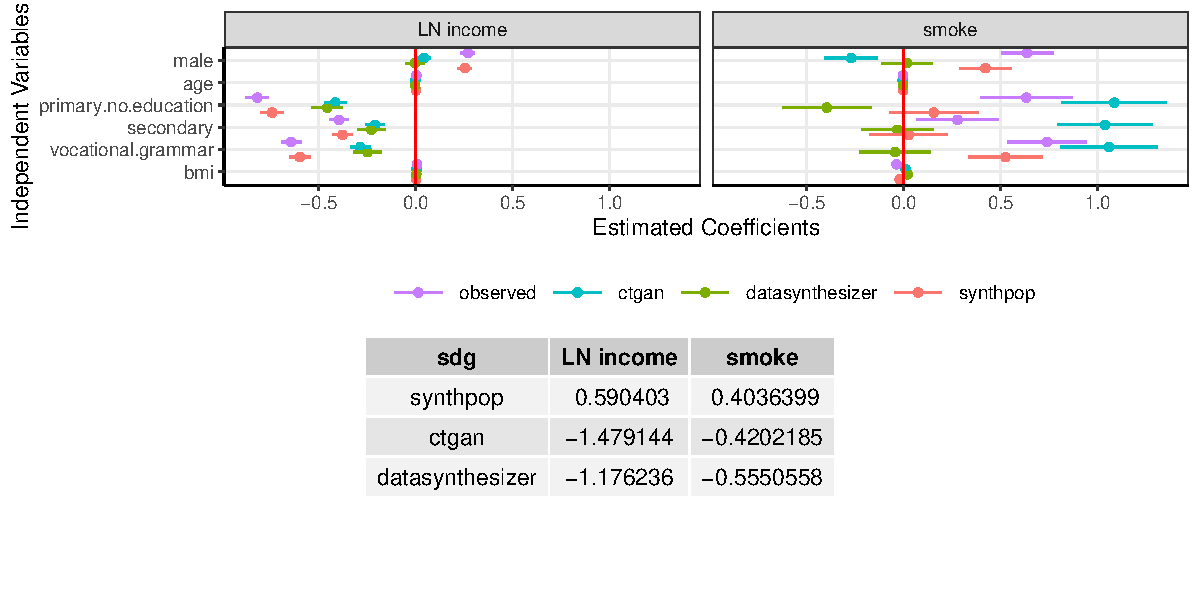
\includegraphics{../graphs/graph_utility_regression_cio_both.pdf}}
    \label{fig:utility_compare_cio}
\end{figure}


%%%%%%%%%%%%%%%%%%%%%%%%%%%%%%%%
% Bibliography
%%%%%%%%%%%%%%%%%%%%%%%%%%%%%%%%
\clearpage
\bibliographystyle{splncs04}
\bibliography{references}

%%%%%%%%%%%%%%%%%%%%%%%%%%%%%%%%
% Appendix
%%%%%%%%%%%%%%%%%%%%%%%%%%%%%%%%
\clearpage
\appendix
%%%%%%%%%%%%%%%%%%%%%%%%%%%%%%%%%%%%%%
%%%%%%%%%%%%%%%%%%%%%%%%%%%%%%%%%%%%%%
%Table
%%%%%%%%%%%%%%%%%%%%%%%%%%%%%%%%%%%%%%
%%%%%%%%%%%%%%%%%%%%%%%%%%%%%%%%%%%%%%

% \begin{table}[ht]
%     \caption{Versions of Social Diagnosis 2011 (SD2011)}
%     \centering
%     % latex table generated in R 4.3.0 by xtable 1.8-4 package
% Thu Feb  1 15:54:24 2024
\begin{tabular}{lll}
    \toprule
Data & & Description \\ \midrule
SD2011(a) && Raw data \\
SD2011(b) && + Cleaned: Missings are numeric values $<$ 0 and empty categorical cells \\
SD2011(c) && + Drop generated variables (\texttt{bmi} and \texttt{agegr}) \\
    \bottomrule
\end{tabular}

%     \label{table:sd2011_versions}
% \end{table}


%%%%%%%%%%%%%%%%%%%%%%%%%%%%%%%%%%%%%%
% Appendix
% DATASYNTHESIZER
%%%%%%%%%%%%%%%%%%%%%%%%%%%%%%%%%%%%%%
\section{Appendix: DataSynthesizer}\label{appendix:datasynethsizer}
\setcounter{figure}{0}    
\setcounter{table}{0}    
\renewcommand*\thetable{\Alph{section}.\arabic{table}}
\renewcommand*\thefigure{\Alph{section}.\arabic{figure}}
\renewcommand{\theHfigure}{\Alph{section}.\arabic{table}}
\renewcommand{\theHtable}{\Alph{section}.\arabic{figure}}

\begin{figure}[ht]
  \caption{Tuning DataSynthesizer across parents}
  \label{fig:tuning_ds}
  \centering
  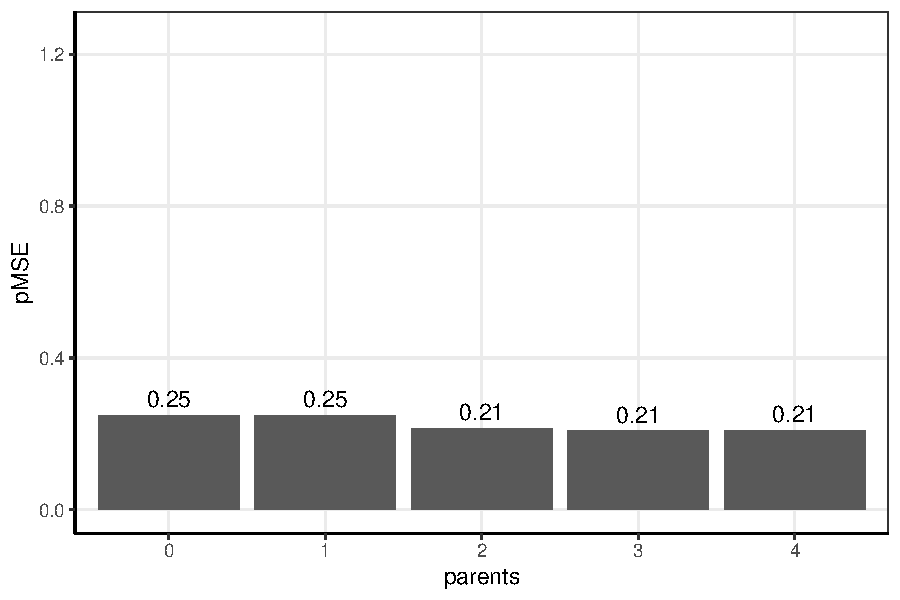
\includegraphics[width=\linewidth]{../graphs/datasynthesizer/datasynthesizer_fidelity_optimize_dataset_parents.pdf}
  \label{fig:tuning_ds_dataset}
\end{figure}

\begin{figure}[ht]
  \caption{Datasynthesizer two-way correlation  (pMSE)}
  \label{fig:ds_fidelity_two_way}
  \centering

  \begin{subfigure}{0.75\textwidth}
    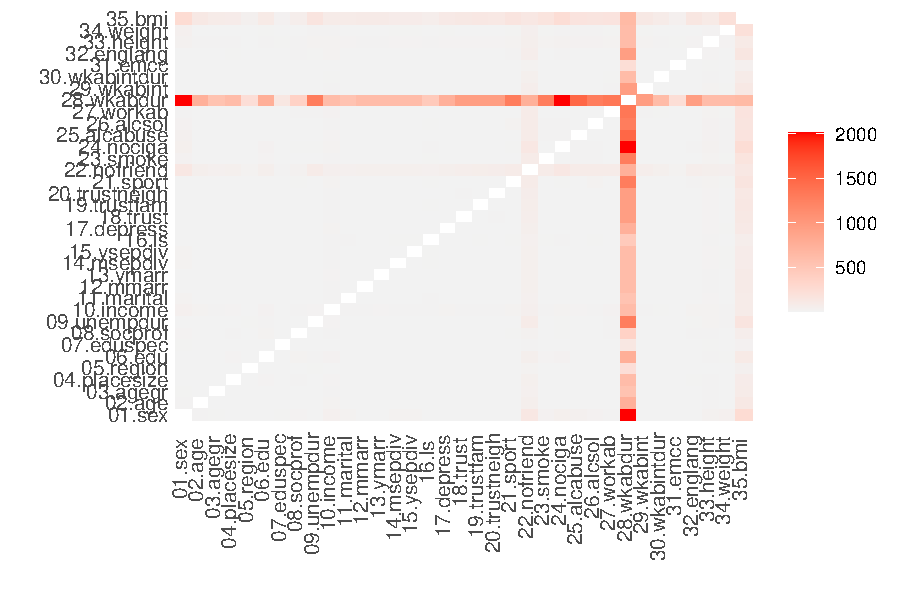
\includegraphics[width=\linewidth]{../graphs/datasynthesizer/datasynthesizer_fidelity_twoway_sd2011.pdf}
    \caption{SD2011(a)}
    \label{subfig:ds_fidelity_two_way_subfig-a}
  \end{subfigure}

  \begin{subfigure}{0.75\textwidth}
    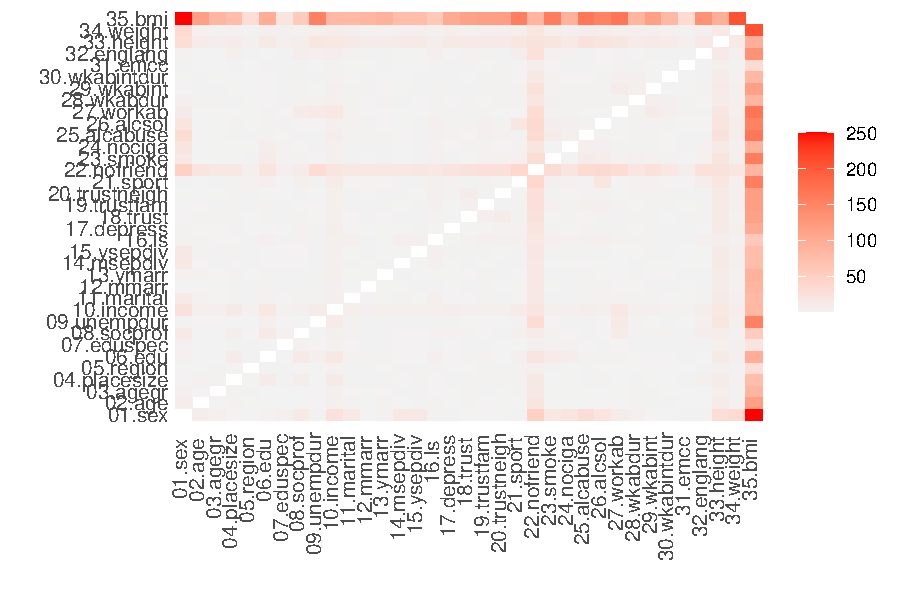
\includegraphics[width=\linewidth]{../graphs/datasynthesizer/datasynthesizer_fidelity_twoway_sd2011_clean.pdf}
    \caption{SD2011(b)}
    \label{subfig:ds_fidelity_two_way_subfig-b}
  \end{subfigure}

  \begin{subfigure}{0.75\textwidth}
    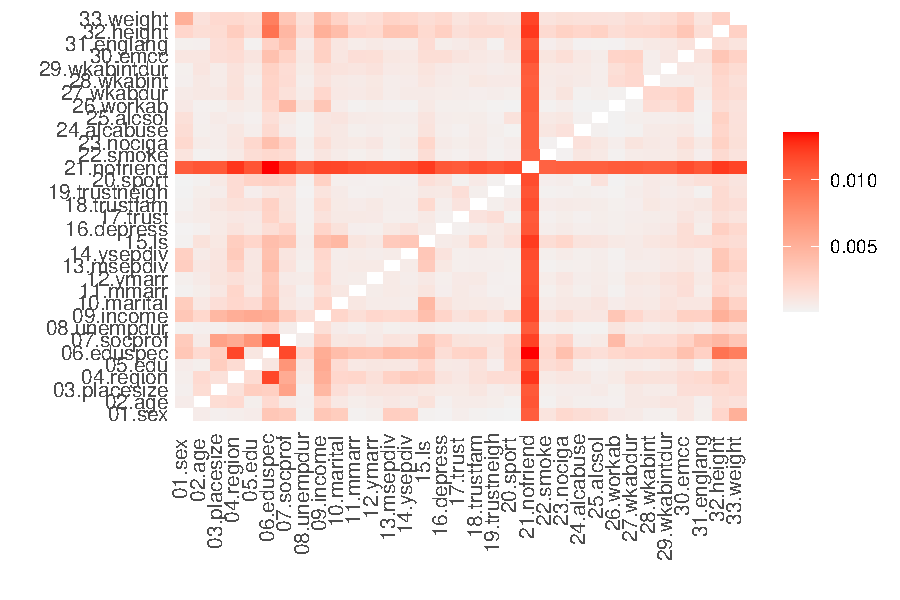
\includegraphics[width=\linewidth]{../graphs/datasynthesizer/datasynthesizer_fidelity_twoway_sd2011_clean_small.pdf}
    \caption{SD2011(c)}
    \label{subfig:ds_fidelity_two_way_subfig-c}
  \end{subfigure}
\end{figure}

\begin{figure}[ht]
  \caption{Frequency values for original and synthetic data (DataSynthesizer)}
  \label{fig:ds_variables}
  \centering

\begin{subfigure}{\textwidth}
    \caption{Variable: \texttt{wkabdur} (Work abroad duration)}
    \resizebox{\textwidth}{!}{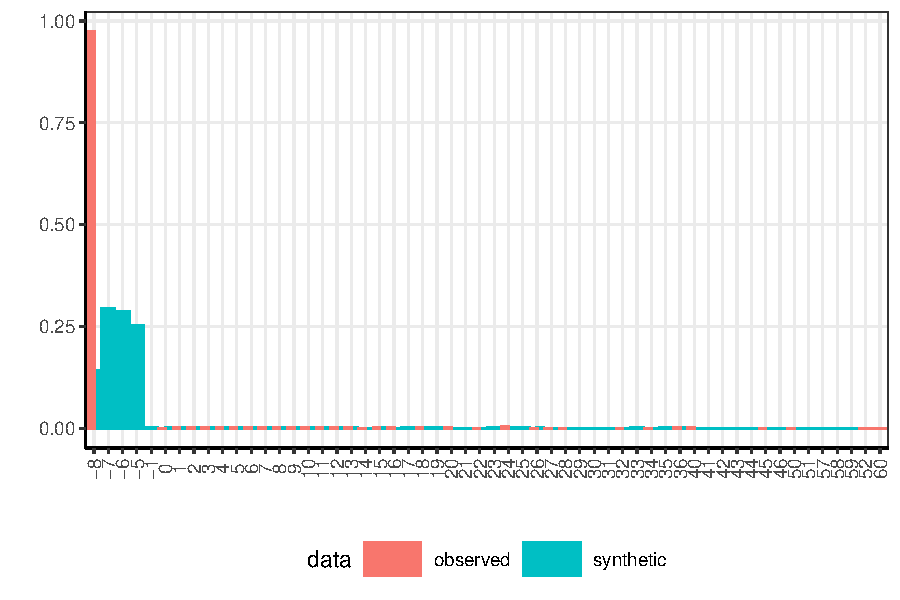
\includegraphics{../graphs/datasynthesizer/datasynthesizer_wkabdur.pdf}}
    \label{subfig:ds_variable_wkabdur}
\end{subfigure}

\begin{subfigure}{\textwidth}
    \caption{Variable: \texttt{bmi} (Body mass index)}
    \resizebox{\textwidth}{!}{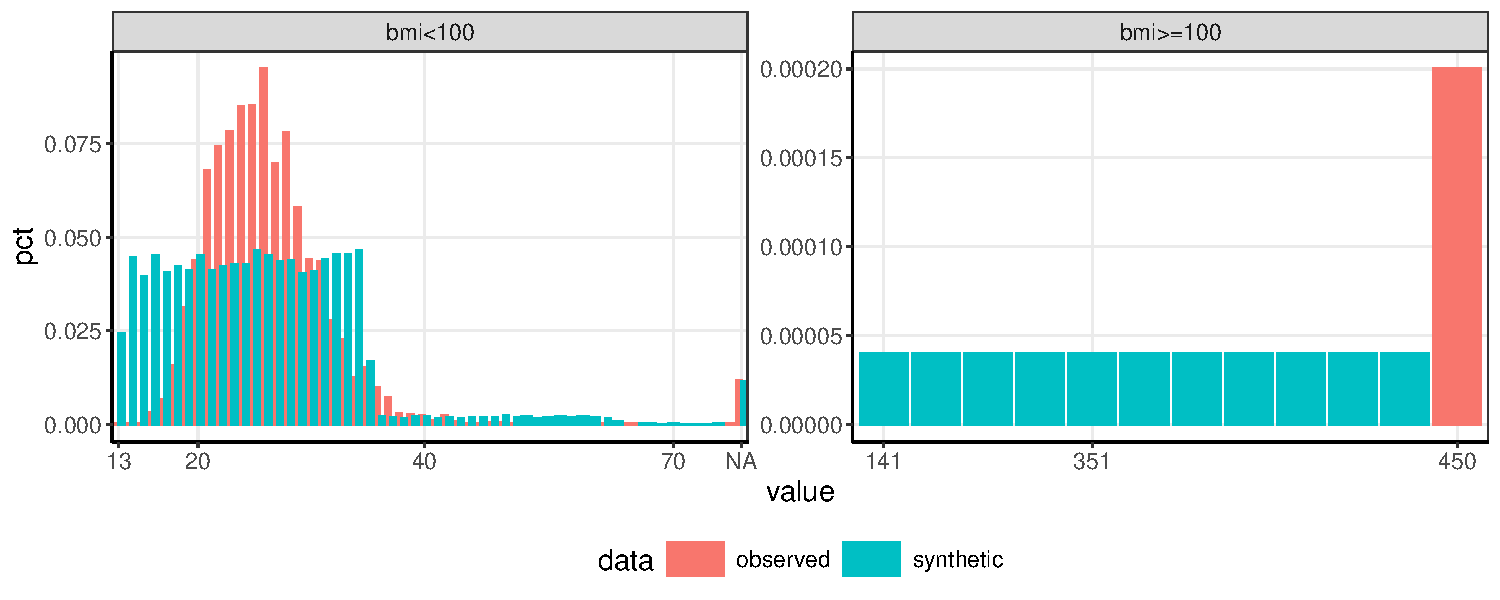
\includegraphics{../graphs/datasynthesizer/datasynthesizer_bmi.pdf}}
    \label{subfig:ds_variable_bmi}
\end{subfigure}


\begin{subfigure}{\textwidth}
    \caption{Variable: \texttt{nofriend} (Number of friends)}
    \resizebox{\textwidth}{!}{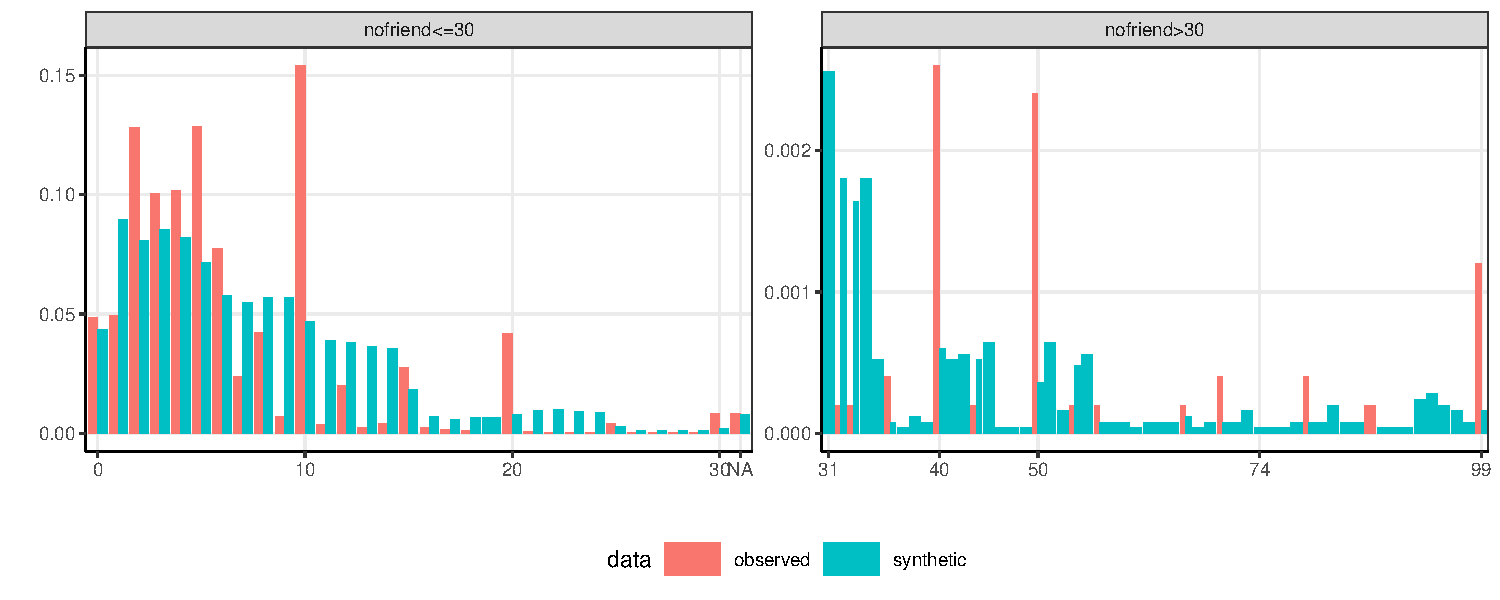
\includegraphics{../graphs/datasynthesizer/datasynthesizer_nofriend.pdf}}
    \label{subfig:ds_variable_nofriend}
\end{subfigure}
\end{figure}

\begin{figure}[ht]
  \caption{Tuning DataSynthesizer across data sets (parents = 2)}
  \label{fig:tuning_ds}
  \centering
  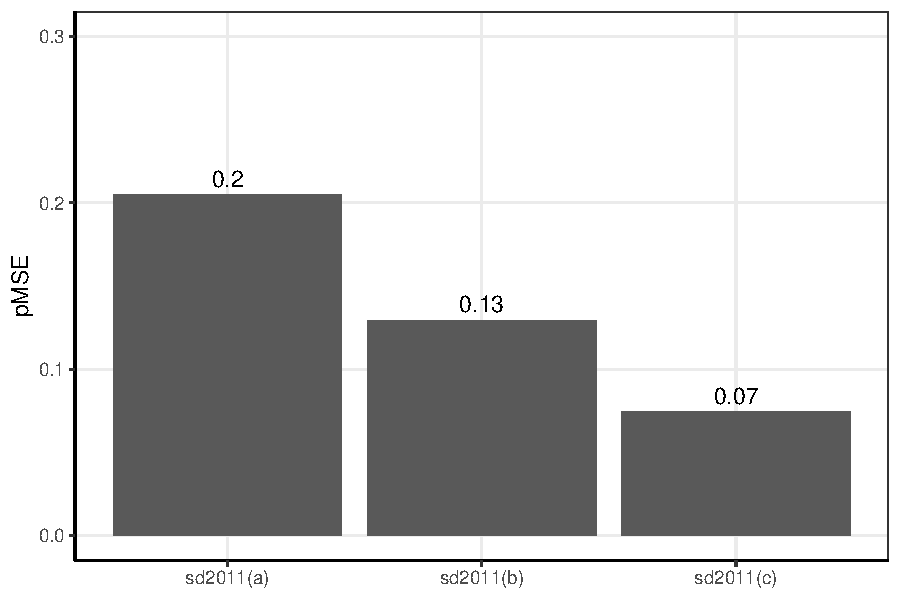
\includegraphics[width=\linewidth]{../graphs/datasynthesizer/datasynthesizer_fidelity_optimize_dataset_compare.pdf}
  \label{fig:tuning_ds_optimize_dataset_compare}
\end{figure}


%%%%%%%%%%%%%%%%%%%%%%%%%%%%%%%%%%%%%%
% Appendix
% CTGAN
%%%%%%%%%%%%%%%%%%%%%%%%%%%%%%%%%%%%%%
\clearpage
\section{Appendix: CTGAN}\label{appendix:CTGAN}
\setcounter{figure}{0}    
\setcounter{table}{0}    
\renewcommand*\thetable{\Alph{section}.\arabic{table}}
\renewcommand*\thefigure{\Alph{section}.\arabic{figure}}
\renewcommand{\theHfigure}{\Alph{section}.\arabic{table}}
\renewcommand{\theHtable}{\Alph{section}.\arabic{figure}}

\begin{table}[!h]
    \rowcolors{1}{white}{lightgray}
    \caption{Batch size and epochs = total steps}
    \centering
    \begin{tabular}{cllll>{\cellcolor{white}}p{1in}}
    % {cllllp{1in}}
    \toprule
    N & Batch size & Steps per Epoch & Epochs & Total Steps & Compare \\
    \midrule
    5.000 & 500 & 10 & 100 & 1,000 & \multirow{4}{1in}{Constant batch size, as shown in figure \ref{subfig:ctgan_fidelity_optimize_batch_size}}\\
    5.000 & 500 & 10 & 300 & 3,000 \\
    5.000 & 500 & 10 & 600 & 6,000 \\
    5.000 & 500 & 10 & 900 & 9,000 \\ \hline
    5.000 & 100 & 50 & 60 & 3,000  & \multirow{4}{1in}{Constant batch size, as shown in figure \ref{subfig:ctgan_fidelity_optimize_epochs}} \\
    5.000 & 250 & 20 & 150 & 3,000 \\
    5.000 & 500 & 10 & 300 & 3,000 \\
    5.000 & 1.000 & 5 & 600 & 3,000 \\ 
    \bottomrule
    \end{tabular}
\end{table}

\begin{figure}[ht]
  \caption{Tuning CTGAN (effect of steps)}
  \label{fig:ctgan_fidelity_optimize}
  \centering

  \begin{subfigure}{0.75\textwidth}
  \caption{Effect of batch size with constant steps (3.000)}
  \resizebox{\textwidth}{!}{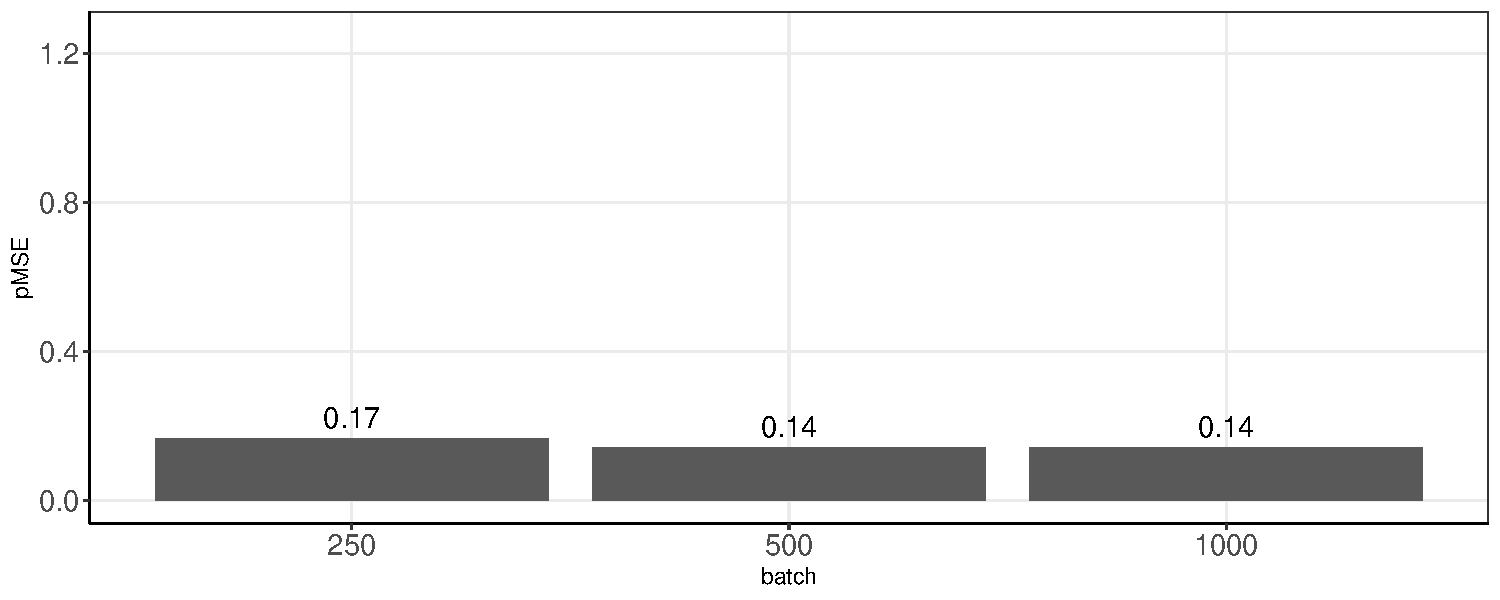
\includegraphics{../../ctgan/graphs/ctgan/ctgan_fidelity_optimize_batch_size.pdf}}
  \label{subfig:ctgan_fidelity_optimize_batch_size}
  \end{subfigure}

  \begin{subfigure}{0.75\textwidth}
  \caption{Effect of epoch number with constant batch size (500)}
  \resizebox{\textwidth}{!}{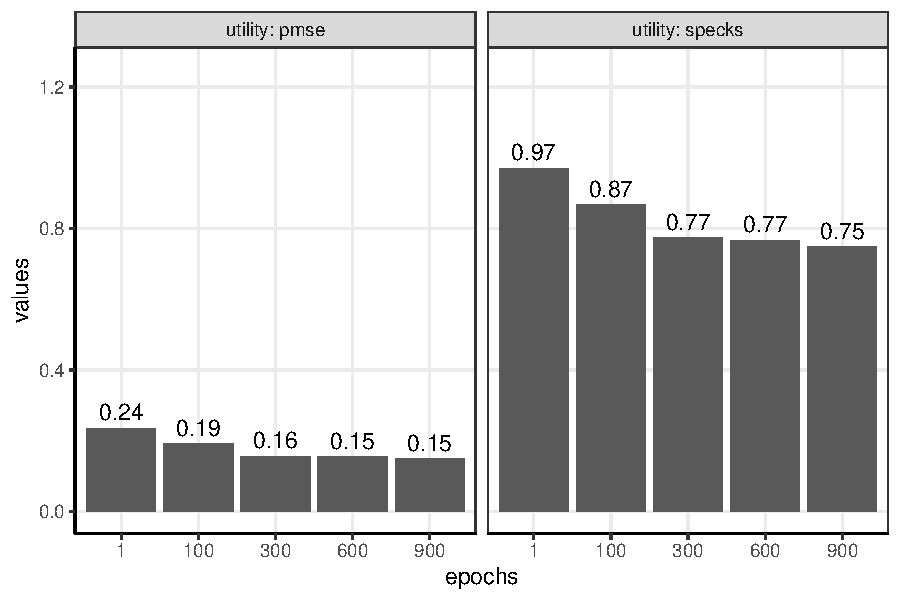
\includegraphics{../../ctgan/graphs/ctgan/ctgan_fidelity_optimize_epochs.pdf}}
  \label{subfig:ctgan_fidelity_optimize_epochs}
  \end{subfigure}

  \begin{subfigure}{0.75\textwidth}
    \caption{Effect of dimensionality}
      \resizebox{\textwidth}{!}{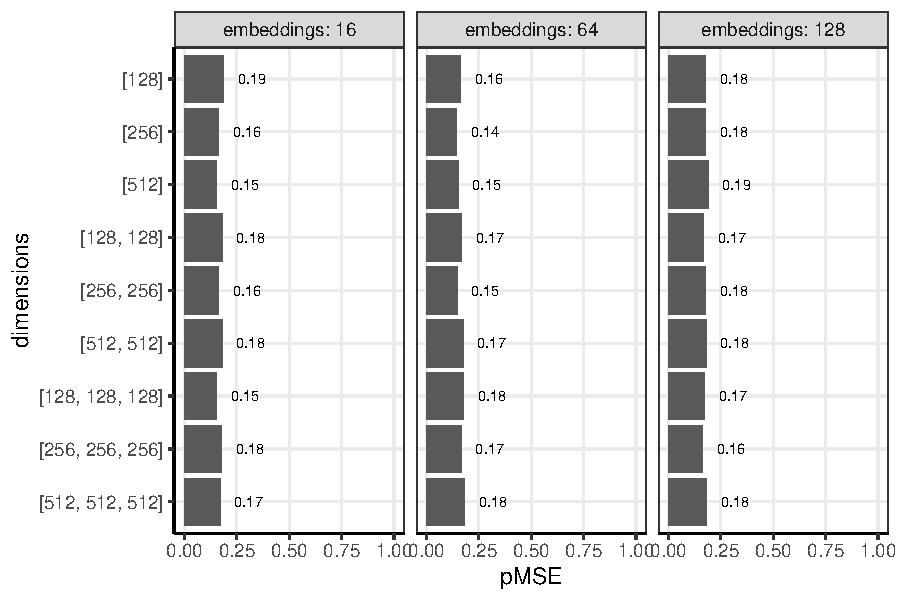
\includegraphics{../../ctgan/graphs/ctgan/ctgan_fidelity_optimize_dimensions.pdf}}
      \label{subfig:ctgan_fidelity_optimize_dimensions}
  \end{subfigure}
\end{figure}


\begin{figure}[ht]
  \caption{CTGAN two-way correlation (pMSE)}
  \label{fig:ctgan_fidelity_two_way}
  \centering

  \begin{subfigure}{0.75\textwidth}
    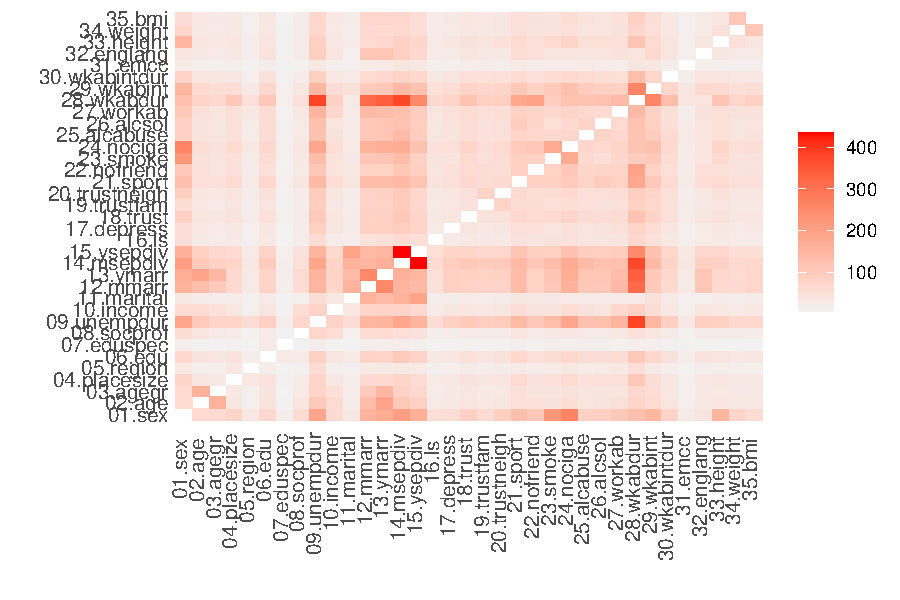
\includegraphics[width=\linewidth]{../graphs/ctgan/ctgan_fidelity_twoway_sd2011.pdf}
    \caption{SD2011(a)}
    \label{fig:ctgan_fidelity_two_way_subfig-a}
  \end{subfigure}

  \begin{subfigure}{0.75\textwidth}
    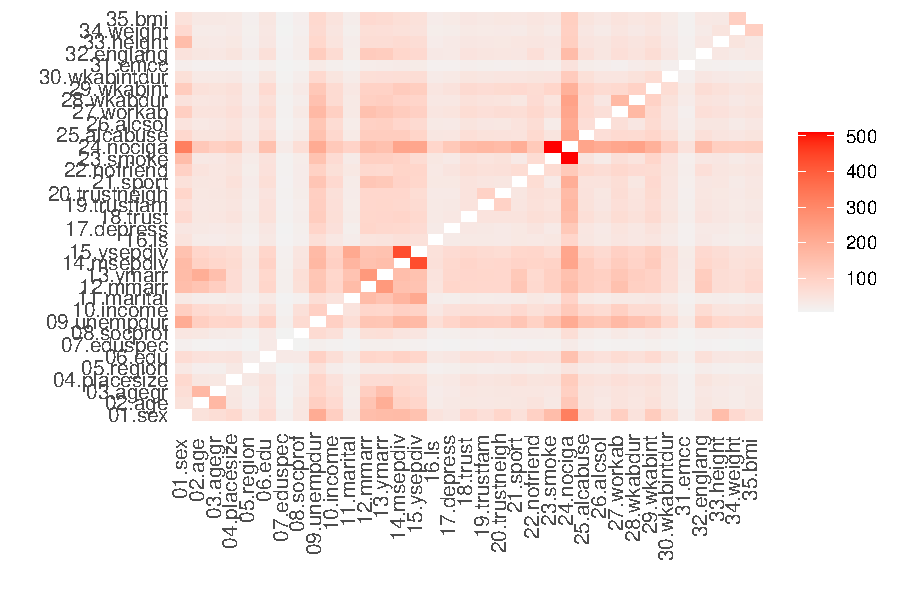
\includegraphics[width=\linewidth]{../graphs/ctgan/ctgan_fidelity_twoway_sd2011_clean.pdf}
    \caption{SD2011(b)}
    \label{fig:ctgan_fidelity_two_way_subfig-b}
  \end{subfigure}

  \begin{subfigure}{0.75\textwidth}
    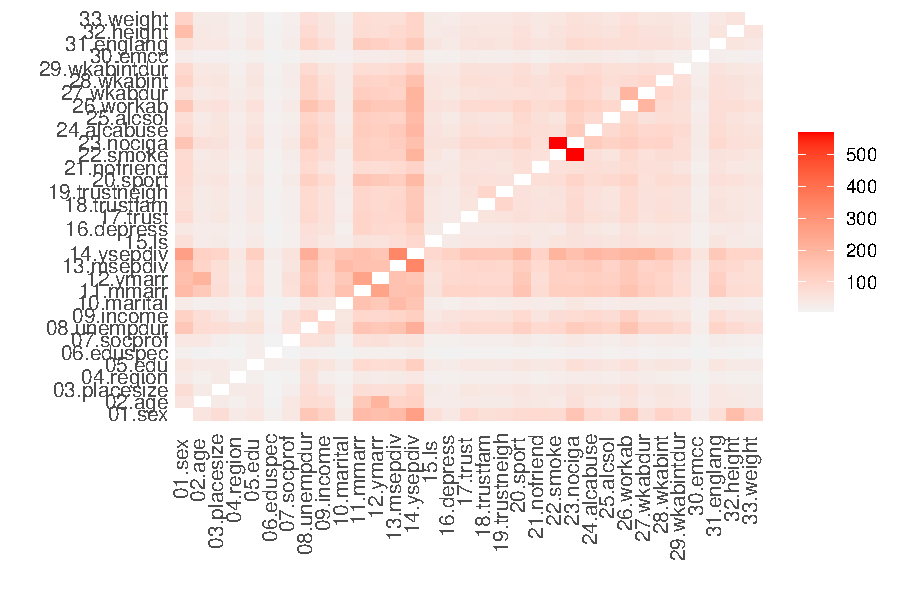
\includegraphics[width=\linewidth]{../graphs/ctgan/ctgan_fidelity_twoway_sd2011_clean_small.pdf}
    \caption{SD2011(c)}
    \label{fig:ctgan_fidelity_two_way_subfig-c}
  \end{subfigure}

\end{figure}

%%%%%%%%%%%%%%%%%%%%%%%%%%%%%%%%%%%%%%
%%%%%%%%%%%%%%%%%%%%%%%%%%%%%%%%%%%%%%
%SYNTHPOP
%%%%%%%%%%%%%%%%%%%%%%%%%%%%%%%%%%%%%%
%%%%%%%%%%%%%%%%%%%%%%%%%%%%%%%%%%%%%%
\begin{figure}[ht]
  \caption{Synthpop two-way correlation  (pMSE)}
  \label{fig:synthpop_fidelity_two_way}
  \centering

  \begin{subfigure}{0.75\textwidth}
    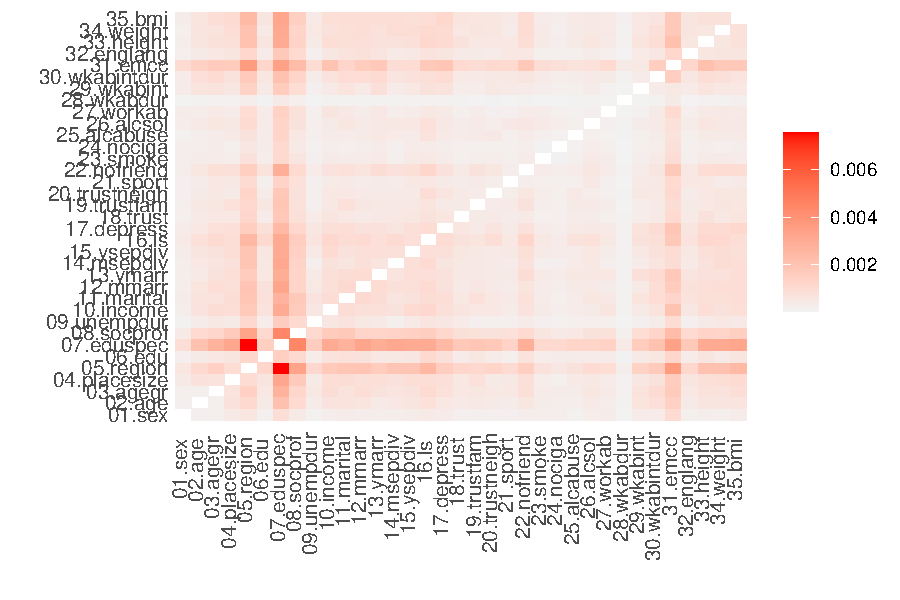
\includegraphics[width=\linewidth]{../graphs/synthpop/synthpop_fidelity_twoway_sd2011.pdf}
    \caption{SD2011(a)}
    \label{fig:synthpop_fidelity_two_way_subfig-a}
  \end{subfigure}

  \begin{subfigure}{0.75\textwidth}
    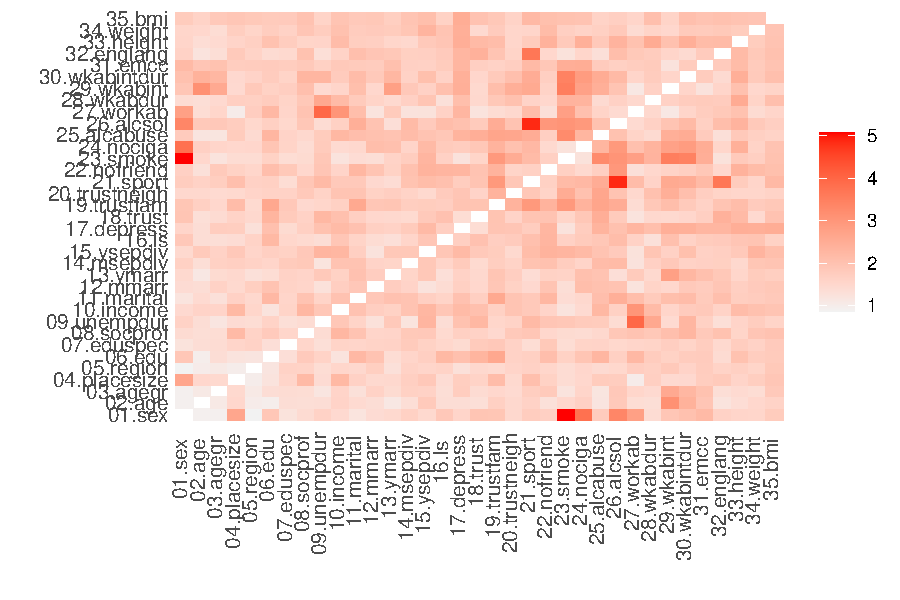
\includegraphics[width=\linewidth]{../graphs/synthpop/synthpop_fidelity_twoway_sd2011_clean.pdf}
    \caption{SD2011(b)}
    \label{fig:synthpop_fidelity_two_way_subfig-b}
  \end{subfigure}

  \begin{subfigure}{0.75\textwidth}
    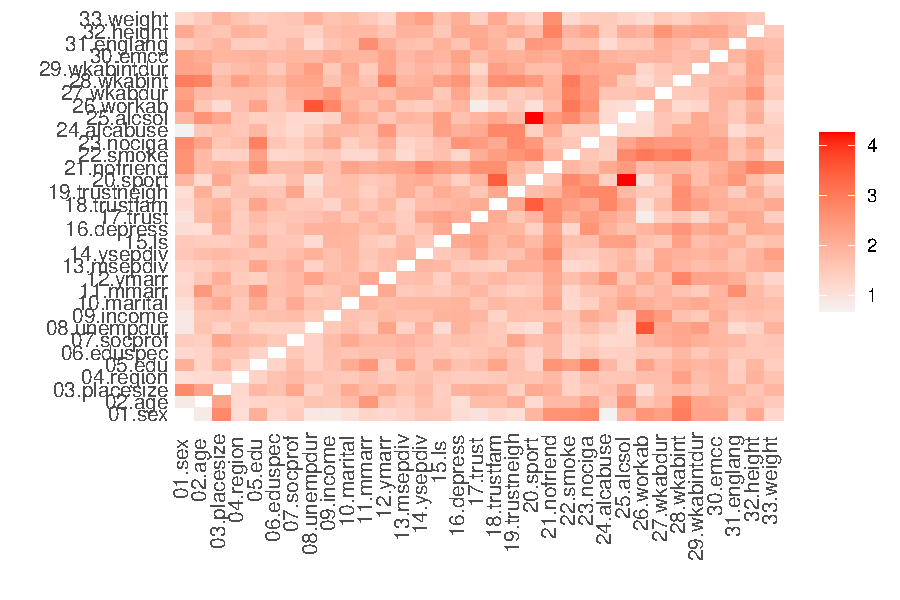
\includegraphics[width=\linewidth]{../graphs/synthpop/synthpop_fidelity_twoway_sd2011_clean_small.pdf}
    \caption{SD2011(c)}
    \label{fig:synthpop_fidelity_two_way_subfig-c}
  \end{subfigure}

\end{figure}



\end{document}
